\documentclass[a4paper]{report}
\usepackage[T1]{fontenc}
\usepackage[utf8]{inputenc}
\usepackage{amsmath}
\usepackage{amsfonts}
\usepackage{amssymb}
\usepackage{graphicx}
\usepackage{dsfont}
\usepackage{framed}
\usepackage{float}
\usepackage{xcolor}
\usepackage[framed]{ntheorem}
\usepackage[french]{babel}
\usepackage{csquotes}
\usepackage{bbold}
\usepackage{subcaption}
\usepackage[export]{adjustbox}
%\usepackage[backend=biber,style=alphabetic,sorting=ynt]{biblatex}
\usepackage[hidelinks]{hyperref}
%\addbibresource{biblio.bib}

\usepackage{fancyhdr}
\pagestyle{fancy}
\renewcommand\headrulewidth{1pt}
\fancyhead[L]{Projet cycleGAN 2020}
\fancyhead[R]{CentraleSupélec}





%\author{Paulin Brissonneau \and Thomas Kebaili \and Ilyas Moutawwakil \and Valentin Laurent \and Lilian Lecomte}
%\date{\today}
%\title{Rapport sur le Projet CycleGan}

\newcommand{\HRule}{\rule{\linewidth}{0.5mm}}

\begin{document}

\begin{titlepage}
  \begin{sffamily}
  \begin{center}

    \textsc{\Large CentraleSupélec}\\[2cm]
    
    \textsc{\huge Rapport de projet}\\[1cm]

	\HRule \\[0.55cm]
    \textsc{\Huge CycleGAN \\[0.2cm] \huge Transformer les chevaux\\en zèbres}\\[0.6cm]
	\HRule \\[3cm]
    
 
  
    \textsc{\large Paulin Brissonneau\\
    	Thomas Kebaili\\
    	Valentin Laurent\\
    	Lilian Lecomte\\
    	Ilyas Moutawwakil}\\[1cm]
        
    \textsc{\large Professeurs encadrants :\\
        Joanna Tomasik\\
        Arpad Rimmel}\\


    \vfill
	{\textsc{\large\today}}
  \end{center}
  \end{sffamily}
\end{titlepage}


%\maketitle

\tableofcontents

\chapter*{Introduction}
\addcontentsline{toc}{chapter}{Introduction}


L'objectif de ce projet est de comprendre, maîtriser, et utiliser la technologie des cycleGAN, proposée par Zhu et al. \cite{zhu_unpaired_2018} en 2017. Un cycleGAN est un algorithme particulier de traitement des images, qui prend la forme d'un réseau de neurones. La problématique à laquelle répond le cycleGAN est celle du transfert de style, cela signifie que l'on cherche à travailler une donnée structurée pour en modifier l’apparence globale. Par exemple, la transformation des objets d'une image, le changement de style pictural ainsi que le changement de style musical sont des transferts de style, et peuvent être abordés par l'utilisation d'un cycleGAN. C'est un problème particulièrement difficile pour un algorithme, en particulier lorsque les données ne sont pas appairées d'un style à un autre.\\

Le projet s'articule autour des cycleGAN, cependant ceux-ci reposent grandement sur la famille d'algorithmes des GAN introduite par Ian Goodfellow \cite{goodfellow_generative_2014-1}, qui reposent eux-même sur beaucoup d'autres concepts de \textit{machine learning}. C'est pourquoi, pour comprendre les cycleGAN, nous devons d'abord passer par plusieurs autres étapes importantes. Nous poserons d'abord les bases du \textit{machine learning}, en partant du simple \textbf{perceptron multicouches (Chapitre 1)}. Ensuite nous étudierons la spécificité des \textbf{couches à convolutions, ou 
CNN (Chapitre 2)} indispensables au traitement des données structurées compositionnelles telles que les images, et développées notamment par Yann LeCun \cite{lecun_gradient-based_1998}. Puis nous nous intéresserons aux \textbf{GAN ou Réseaux Adverses Génératifs (Chapitre 3)}. Il existe plusieurs architectures de GAN, nous en verrons les deux types principaux : les DCGAN proposés par Radford et al. en 2016 \cite{radford_unsupervised_2016} et les W-GAN proposés par Arjovsky et al. en 2017 \cite{arjovsky_wasserstein_2017}. Enfin, grâce à tous ces outils, nous pourrons comprendre le fonctionnement des \textbf{cycleGAN (Chapitre 4)}. Nous chercherons ensuite à appliquer notre cycleGAN au remplissage d'images (image painting). L'idée de base est de retirer par exemple un individu d'une photo. Pour ceci, nous étudierons le \textbf{MaskRCNN (Chapitre 5)} permettant d'identifier dans l'image la zone à retirer. Tous ces points sont accompagnés de l'implémentation des algorithmes sur TensorFlow 2.0 \cite{goldsborough_tour_2016}.\\

Ce rapport constitue un résumé des connaissances que nous avons acquises.

\chapter{Multi-Layer Perceptron}

\section{Les neurones}

Les technologies qui vont êtres présentées dans la suite se basent toutes sur l'idée de neurone artificiel, aussi appelé neurone formel. McCulloh et Pitts le formalise en 1943 \cite{mcculloch_logical_1943}.
Un neurone formel est composé de deux parties.\begin{itemize}
\item La première consiste à faire la somme pondérée par des poids des valeurs d'entrée du neurone auxquelles on peut éventuellement ajouter un biais. Les poids sont propres au neurone et il y a un poids par entrée.
\item La deuxième partie du neurone est la fonction d'activation. Cette fonction va s'appliquer sur le résultat de la somme pondérée. On choisit quasi-exclusivement des fonctions non-linéaires pour deux raisons : briser la linéarité (car dans le cas contraire le réseau serait assimilable à une seule matrice) et obtenir un résultat d'une certaine forme (par exemple une probabilité entre 0 et 1).
\end{itemize}
McCulloh et Pitts dans leur première ébauche du neurone formel considérèrent des neurones au résultat binaire à l'aide d'une fonction d'activation de Heavyside. Un tel neurone formel est représenté par la figure \ref{neurone_exemple}.



\begin{figure}[!h]
\centering
\includegraphics[width=300pt,valign=t]{"images/MLP/neurone_exemple2"}
\caption{Exemple de neurone dont les poids sont les coefficents $w_1$ à $w_2$, et le biais est $w_0$. La fonction de Heavyside s'applique à la somme pour donner une sortie du neurone dans $\{0, 1\}$. Cette image provient d'un article de Benharir et al. \cite{benharir_approche_2014}.}
\label{neurone_exemple}
\end{figure}

Ainsi formellement en utilisant les notant $X = \begin{pmatrix} x_1\\ \vdots \\ x_n \end{pmatrix}$  les entrées du neurone, $W = \begin{pmatrix} w_1\\ \vdots \\ w_n \end{pmatrix}$ les poids correspondants et $\varphi$ la fonction d'activation, $b$ le biais, un neurone correspond à une fonction $N$ telle que : $$N(x_1,...,x_n,w_1,...,w_n) = \varphi(b+ \sum\limits_{i} x_i w_i) = \varphi(W^T  X+b)$$



\section{Le perceptron}
En 1958, Frank Rosenblatt utilise l'idée des neurones artificiels pour inventer le perceptron \cite{rosenblatt_perceptron_1958}. Son idée est d'utiliser les neurones pour reconnaître des formes simples dans des images. Cependant dans cette forme simple, il conserve les neurones tels que définis en 1943 avec la fonction de Heavyside et une seule couche de neurones (c'est-à-dire que les différents neurones ne sont pas reliés entre eux). Cela limite l'intérêt du perceptron : il ne peut apprendre que des \textit{pattern} linéairement séparables. Minsky démontre par exemple que le perceptron est incapable d'effectuer un XOR \cite{minsky_perceptrons_2017}. L'idée est d'ajuster les poids pour que la sortie du neurone soit 1 si et seulement si l'entrée est dans l'ensemble que l'on cherche à reconnaître. Le schéma d'un perceptron est donné sur la figure \ref{perceptron}.

\begin{figure}[!h]
\centering
\includegraphics[width=250pt,valign=t]{"images/MLP/perceptron"}
\caption{Exemple de perceptron à $n$ entrées et $p$ sorties. Il peut donc servir de classificateur à $p$ classes.}
\label{perceptron}
\end{figure}

\section{Perceptron multicouche}
Un \textbf{perceptron multicouche}, \textbf{mutliperceptron}, ou \textbf{MLP} (pour \textit{Multi-Layer Perceptron}) est composé de différentes couches: \begin{itemize}
\item La couche d'entrée qui correspond aux valeurs des données.
\item Une couche de sortie qui correspond aux valeurs renvoyées par le MLP.
\item Une ou plusieurs couches cachées (\textit{hidden layers}) qui sont des couches de neurones reliées entre elles. À chaque couche, les sorties correspondent aux entrées de la couche suivante.

\end{itemize}

Écrivons formellement ceci. On définit $N$ la sortie de la $i^e$ couche :
$$N^{(i)}  = \begin{pmatrix} 1\\ n_1^{(i)}\\ \vdots \\ n_{p_i}^{(i)} \end{pmatrix}$$  Le 1 permet la présence d'un biais.\\ 
Définissons également $W^{(i)}$ la matrice des poids de la couche i.

$$W^{(i)} = \begin{pmatrix} w_{1,1}^{(i)}& \hdots & w_{1, p_i}^{(i)} \\  \vdots & \ddots &  \vdots \\ w_{p_i1}^{(i)} & \hdots & w_{p_ip_i}^{(i)} \end{pmatrix}$$

Soit $\varphi_k^{(i)}$ la fonction d'activation de ce même neurone et $\Phi^{(i)}((x_1,...,x_{p_i})) \to (\varphi_1^{(i)}(x_1), ... \varphi^{(i)}_{p_i}(x_{p_i}))$.\\

On notera que si le réseau possède $L+1$ couches (de $0$ à $ L$), $N^{(0)} = X$ et $N^{(L)} = Y$. Dès lors, $$\forall i \in [1,L], N^{(i)} = \Phi^{(i)}(W^{(i)}N^{(i-1)}). $$





\subsection{Quelques fonctions d'activation}
Il existe de nombreuses fonctions d'activation avec chacune leurs avantages et leurs défauts. En voici quelques-unes.

\subsubsection{Sigmoïde}
Cette fonction permet d'avoir des valeurs de sortie entre 0 et 1 mais souffre d'un problème de \textit{gradient vanishing}, c'est-à-dire que proche de sa zone de saturation le gradient sera très vite trop faible. Cela portera défaut à l'apprentissage lors de l'application de la rétropropagation du gradient. La fonction introduit un hyperparamètre $\lambda$. Son allure est donnée par la figure \ref{sigmoide}.

\begin{displaymath}
\varphi_\lambda (x) = \frac{1}{1+e^{-\lambda x}}
\end{displaymath}

\begin{figure}[!h]
\centering
\includegraphics[width=150pt]{"images/MLP/sigmoide2"}
\caption{Fonction sigmoïde\\}
\label{sigmoide}
\end{figure}


\subsubsection{Tangente hyperbolique}
Cette fonction permet d'avoir des valeurs de sortie entre -1 et 1. Elle souffre du même problème de \textit{gradient vanishing} que la sigmoïde. Son allure est donnée par la figure \ref{tanh}.
\begin{displaymath}
\varphi (x) = tanh(x)
\end{displaymath}

\begin{figure}[!h]
\centering
\includegraphics[width=150pt]{"images/MLP/tanh2"}
\caption{Fonction tangente hyperbolique\\ }
\label{tanh}
\end{figure}


\subsubsection{Softmax}
Cette fonction s'applique sur un vecteur, elle est souvent utilisée en sortie car elle permet d'obtenir des sorties homogènes à des probabilités (entre 0 et 1 et dont la somme sur les sorties vaut 1).
\begin{displaymath}
\varphi_\lambda (X)_j = \frac{e^{-x_j}}{\sum\limits_{k}  e^{-x_k}}
\end{displaymath}

\subsubsection{ReLu}
La ReLu (pour \textit{Rectified Linear Unit}) définie ci-dessous permet d'éviter le \textit{gradient vanishing} puisqu'elle ne possède pas de zone de saturation. Son inconvénient réside dans sa partie de gradient nul. En effet, si sa pré-activation (la somme pondérée de ses entrées) est négative, l'effet du neurone sur les couches suivantes sera nul. Autrement, le gradient de l'erreur commise par ce neurone sera nul, il ne pourra donc pas mettre à jour ses poids et restera dans cette position pendant tout l'apprentissage. On dit que le neurone \textit{meurt}. L'allure de la ReLu est donnée par la figure \ref{ReLu}.

\begin{displaymath}
\varphi (x) = max(0,x)
\end{displaymath}

\begin{figure}[!h]
\centering
\includegraphics[width=150pt]{"images/MLP/reLu2"}
\caption{Fonction reLu}
\label{ReLu}
\end{figure}

\subsubsection{Et bien d'autres...}
Il existe beaucoup d'autres fonctions d'activation ayant divers effets. Ce champ de recherche est très actif : de nouvelles fonctions sont découvertes chaque année dont l'effet n'est pas toujours bien compris. On peut par exemple citer la fonction Mish (2019) \cite{misra_mish_2019-1} ou la softexponentielle(2016)  \cite{godfrey_continuum_2016}.

\begin{figure}[!h]
\centering
\includegraphics[width=150pt]{"images/MLP/mish2"}
\caption{Fonction Mish}
\label{Mish}
\end{figure}


\section{Rétropropagation}
\subsection{Principe}

On définit une fonction de coût $J$. Cette fonction mesure l'écart entre ce que renvoie notre MLP et ce qu'il devrait renvoyer. Notre objectif est donc de la minimiser afin d'obtenir la plus grande précision possible. Pour cela on va agir sur les seuls paramètres modifiables : les poids. On va ainsi calculer le gradient $\nabla J$ à l'aide des dérivées partielles par rapport aux poids de la dernière couche de neurones. Dès lors, par la règle de la chaîne, on peut calculer les dérivées partielles par rapport aux poids de la couche précédente et ainsi de suite. Ces dérivées partielles seront utilisées par les algorithmes d'optimisation pour minimiser $J$ en mettant à jour les poids par itérations successives. Le principe de la rétropropagation de l'erreur est illustré par la figure \ref{backward}.

\begin{figure}[!h]
\centering
\includegraphics[width=160pt]{"images/MLP/forward"}
\hspace*{5mm}
\includegraphics[width=160pt]{"images/MLP/backward"}
\caption{Principe de la rétropropagation du gradient. À gauche, la propagation avant, qui permet de calculer la sortie du réseau en fonction de l'entrée. À droite, la rétropagation de l'erreur, qui permet de calculer l'influence de chaque poids sur l'erreur en sortie. Ces deux schémas proviennent d'un article de Lillicrap et al. \cite{lillicrap_backpropagation_2020}}.
\label{backward}
\end{figure}

\subsection{Les fonctions de coûts}
Il en existe plusieurs, voici les principales.

\subsubsection{Mean Absolute Error}
Cette fonction compte les erreurs proportionnellement à leur importance.
\begin{displaymath}
MAE = \frac{1}{n} \sum\limits_{i = 0}^{n} |y_{th} - y_{mes}|
\end{displaymath}

où $y_{th}$ est la sortie théorique, et $y_{mes}$ est la sortie prédite par l'algorithme.

\subsubsection{Mean Squared Error}
Parfois, on est prêt à tolérer de faibles erreurs mais on refuse catégoriquement les aberrations. C'est exactement ce que fait l'erreur quadratique moyenne. Elle attribue un poids beaucoup plus important aux grandes déviations.
\begin{displaymath}
MSE = \frac{1}{n} \sum\limits_{i = 0}^{n} (y_{th} - y_{mes})^2
\end{displaymath}

où $y_{th}$ est la sortie théorique, et $y_{mes}$ est la sortie prédite par l'algorithme.

\subsubsection{Entropie croisée}
L'entropie croisée, introduite à l'origine pour mesurer la distance entre deux distributions de probabilités est très efficace pour les réseaux neuronaux dans le cas de la classification. En effet, dans ce cas il s'agit d'approximer une densité de probabilité.

\begin{displaymath}
Cross Entropy = - \sum\limits_{i = 0}^{n} y_{th}  log(y_{mes})
\end{displaymath}

où $y_{th}$ est la classe théorique, et $y_{mes}$ est la classe prédite par l'algorithme.

\subsection{Algorithmes d'optimisation}
La fonction de coût utilisée dans toute cette partie est $J = \sum\limits_{k} (y_{th} - y_{mes})^2$


\subsubsection{Descente de gradient stochastique}
Il s'agit de l'algorithme classique.  $w_{jk}^{(i)} \leftarrow w_{jk}^{(i)} - \alpha \frac{\partial J}{\partial w_{jk}^{(i)}}$ . Un coefficient $\alpha$ appelé \textbf{taux d'apprentissage} définit l'ampleur de la modification du poids. Plus $\alpha$ est grand, plus le pas est important. Ainsi un taux d'apprentissage trop faible entraînera une convergence trop lente ou un blocage dans un minimum local mais un taux trop élevé risque de ne jamais converger. Un exemple d'application de la descente de gradient stochastique est donné par la figure \ref{descentedegradientstochastique}.

\begin{figure}[!h]
\centering
\includegraphics[width=160pt]{"images/MLP/descentedegradientstochastique"}
\hspace*{5mm}
\includegraphics[width=160pt]{"images/MLP/descentedegradientstochastiquepropre"}
\caption{Exemple d'application de la descente de gradient stochastique. La figure représente le cheminement de la valeur des deux poids. La hauteur représente l'erreur. On voit bien ici que l'algorithme peut entraîner un blocage dans un minimum local.}
\label{descentedegradientstochastique}
\end{figure}



\subsubsection{Descente de gradient newtonienne}
Ici, on ajoute un terme d'inertie à la modification du poids cela entraîne l'apparition d'un nouvel hyperparamètre $\beta_1$ qui sert à doser cette inertie. On note $\nu$ le terme de descente au pas précédent : $$ w_j{k}^{(i)} \leftarrow w_{jk}^{(i)} + \beta_1 \nu - \frac{\partial J}{\partial w_{jk}^{(i)}}$$
Un exemple d'application de la descente de gradient stochastique est donné par la figure \ref{descentedegradientnewtonnienne}.
	
\begin{figure}[!h]
\centering
\includegraphics[width=160pt]{"images/MLP/descentedegradientnewtonnienne"}
\hspace*{5mm}
\includegraphics[width=160pt]{"images/MLP/descentedegradientnewtonniennepropre"}
\caption{Exemple d'application de la descente de gradient stochastique. La figure représente le cheminement de la valeur des deux poids. La hauteur représente l'erreur. On remarque que l'algorithme est bien plus instable mais explore plus et ne reste pas forcément bloqué dans les minimum locaux.}
\label{descentedegradientnewtonnienne}
\end{figure}

\subsubsection{RMSProp}
L'algorithme, dont un exemple d'application est donné sur la figure \ref{RMSProp}, est le suivant : on choisit les hyper-paramètres $\beta_2$, $\alpha$, et $\varepsilon$ tel que $\varepsilon$ soit petit mais non nul, on initialise $\nu$ à 0.
A chaque pas on calcule :

\begin{displaymath}
s \leftarrow \beta_2 s + (1-\beta_2)  (\frac{\partial J}{\partial w_{jk}^{(i)}})^2 \\
\end{displaymath}
\begin{displaymath}
w_{jk}^{(i)} \leftarrow w_{jk}^{(i)} - \frac{\alpha}{\sqrt{s+\varepsilon}}\frac{\partial J}{\partial w_{jk}^{(i)}}
\end{displaymath}

\begin{figure}[!h]
\centering
\includegraphics[width=160pt]{"images/MLP/RMSProp"}
\hspace*{5mm}
\includegraphics[width=160pt]{"images/MLP/RMSPropPropre"}
\caption{Exemple d'application de RMSProp. La figure représente le cheminement de la valeur des deux poids. La hauteur représente l'erreur. L'algorithme est sensible aux minima locaux mais peu aux grands gradients.}
\label{RMSProp}
\end{figure}

\subsubsection{ADAM}
Il s'agit d'une combinaison de RMSProp et de la descente de gradient newtonienne.
L'algorithme est le suivant : on choisit les hyperparamètre $\beta_1$, $\beta_2$,  $\alpha$ et $\varepsilon$ tel que epsilon soit petit mais non nul, on initialise $\nu$ et $s$ à 0.
A chaque pas on calcule :
\begin{displaymath}
\nu \leftarrow \beta_1 \nu + (1-\beta_1) \frac{\partial J}{\partial w_{jk}^{(i)}} \\
\end{displaymath}
\begin{displaymath}
s \leftarrow \beta_2 s + (1-\beta_2) (\frac{\partial J}{\partial w_{jk}^{(i)}})^2 \\
\end{displaymath}
\begin{displaymath}
w_{jk}^{(i)} \leftarrow w_{jk}^{(i)} - \frac{\alpha}{\sqrt{s+\varepsilon}}\frac{\partial J}{\partial w_{jk}^{(i)}}
\end{displaymath}
Un exemple d'application est donné sur la figure \ref{ADAM}.

\begin{figure}[!h]
\centering
\includegraphics[width=160pt]{"images/MLP/adam"}
\hspace*{5mm}
\includegraphics[width=160pt]{"images/MLP/adampropre"}
\caption{Exemple d'application de ADAM. La figure représente le cheminement de la valeur des deux poids. La hauteur représente l'erreur. L'algorithme est peu sensible aux minima locaux et beaucoup plus stable que la méthode de descente de gradient newtonnienne.}
\label{ADAM}
\end{figure}



\subsubsection{Comparatif des algorithmes}

Pour comparer les différents algorithmes, nous pouvons représenter sur un seul dessin leurs convergences. Le résultat est présenté par la figure \ref{Comparatifoptimiseurs}.

\begin{figure}[!h]
\centering
\includegraphics[width=220pt]{"images/MLP/comparatifoptimiseurs"}
\caption{Comparaison des 4 algorithmes présentés. La figure représente le cheminement de la valeur des deux poids. La hauteur représente l'erreur. On observe que ADAM est clairement meilleur que les autres.}
\label{Comparatifoptimiseurs}
\end{figure}

\subsection{Les batchs}
Souvent, la dérivée $\frac{\partial J}{\partial w_{jk}^{(i)}}$ n'est pas calculée sur une seule entrée. Afin d'obtenir une estimation plus précise du gradient de $J$, on le moyenne sur $n$ entrées. On appelle cela la méthode par batchs. Il est bon de remarquer que le choix de $n$ n'est pas anodin. Il s'agit ici encore d'un hyper-paramètre à régler qui influe sur la convergence du réseau. L'influence de la taille des batchs sera étudiée plus loin.



\section{Implémentation et résultats}
\subsection{Avant-propos}
Nous avons étudié l'impact de différents hyperparamètres sur les résultats du MLP. Sauf mention contraire, le jeu de données utilisé est MNIST. MNIST est un ensemble d'images en niveau de gris de chiffres écrits à la main. Le MLP est alors utilisé en tant que classificateur. Il doit reconnaître, à partir du niveau de gris des pixels, quel est le chiffre dessiné. La tâche typique de l'algorithme est présentée par une interface simple sur la figure \ref{MNIST_exemple}.\\
Les résultats de précision sont calculés sur un jeu de données de test composé de données choisies aléatoirement avant l’entraînement et n'étant pas utilisées pour celui-ci. Afin de mesurer l'effet des hyperparamètres, on trace toujours les courbes avec tous les hyperparamètres égaux sauf celui qui varient.
Les MLP utilisés pour les mesures ont été réalisés \textit{from scratch}. La configuration à partir de laquelle on fait varier les hyper-paramètres a été obtenue par ajustement par essais-erreurs et ne prétend pas être optimale. Toutefois, les valeurs observées étaient de l'ordre de celles trouvées dans la littérature. Les données sont moyennées sur 50 lancers de l'algorithme et l'intervalle de confiance à 95\% est indiqué.

\begin{figure}[!h]
\centering
\includegraphics[width=200pt]{"images/MLP/MNIST_exemple"}
\caption{Exemple de résultat de classification avec le MLP }
\label{MNIST_exemple}
\end{figure}

\subsection{Effet du nombre de neurones par couche}
On s'intéresse ici à la largeur du réseau, c’est-à-dire-dire le nombre de neurones par couche. Les résultats sont présentés sur la figure \ref{MLP_largeur}. On y observe  à la fois que prendre trop peu de neurones ne permet pas une classification satisfaisante, et à la fois que prendre trop de neurones est contre productif. Il s'agit alors de trouver le juste milieu.

\begin{figure}[!h]
\centering
\includegraphics[width=200pt]{"images/MLP/MLP_largeur"}
\caption{Courbes de précision sur les données de test en fonction de l'avancement de l'apprentissage, en faisant varier le nombre de neurones par couche.\\ }
\label{MLP_largeur}
\end{figure}

\subsection{Effet du nombre de couches de neurones}
On s'intéresse ici à la profondeur du réseau. Les résultats sont présentés sur la figure \ref{MLP_profondeur}. On notera que le cas on l'a une seule couche correspond à un perceptron simple. On observe que le MLP est plus performant que le perceptron simple. Cependant augmenter la profondeur du réseau réseau réduit sa vitesse de convergence.

\begin{figure}[!h]
\centering
\includegraphics[width=200pt]{"images/MLP/MLP_profondeur"}
\caption{Courbes de précision sur les données de test en fonction de l'avancement de l'apprentissage, en faisant varier le nombre de couches du réseau.\\ }
\label{MLP_profondeur}
\end{figure}

\subsection{Taille des batchs}
Comme vu précédemment la taille des batchs influe grandement sur l'algorithme.

\subsubsection{Méthode stochastique}
Il s'agit du cas où le batch est de taille 1. On met à jour les poids pour chaque exemple parcouru. On observe alors sur la figure \ref{batch1} une forte instabilité liée au fait que le gradient peut fortement varier d'un exemple à l'autre.
\begin{figure}[!h]
\centering
\includegraphics[width=200pt]{"images/MLP/batch1"}
\caption{Courbes de précision sur les données de test en fonction de l'avancement de l'apprentissage avec \textit{batch\_size} = 1. Un epoch correspond au passage d'un batch dans l'algorithme. }
\label{batch1}
\end{figure}


\subsubsection{Méthode par batch}
On illustre ici avec de très grands batch. On moyenne le gradient dans cet exemple sur 2048 images. Sur la figure \ref{batch2}, on n'observe plus l'instabilité initiale. Cependant de grands batch augmentent la sensibilité aux minima locaux et mène parfois à une saturation de la fonction de coût. De plus, une passe correspond au passage d'un batch dans l'algorithme. Ainsi, avec de très grands batch, le calcul de chaque pas peut devenir très long. Souvent, une grande taille de batch est associée à un fort taux d'apprentissage (car on estime mieux le gradient).
\begin{figure}[!h]
\centering
\includegraphics[width=200pt]{"images/MLP/batch2048"}
\caption{Courbes de précision sur les données de test en fonction de l'avancement de l'apprentissage avec \textit{batch\_size} = 2048. Un epoch correspond au passage d'un batch dans l'algorithme. }
\label{batch2}
\end{figure}

\subsubsection{Méthode par mini-batch}
On choisit des batch de taille plus restreinte (ici 32 images). On réduit l'instabilité pour qu'elle ne gêne pas trop la convergence, de plus le coût de calcul reste raisonnable. Enfin on garde une légère instabilité qui rend l'algorithme plus résistant aux minima locaux. Le résultat est présenté sur la figure \ref{batch3}.

\begin{figure}[!h]
\centering
\includegraphics[width=200pt]{"images/MLP/batch32"}
\caption{Courbes de précision sur les données de test en fonction de l'avancement de l'apprentissage avec \textit{batch\_size} = 32. Un epoch correspond au passage d'un batch dans l'algorithme. }
\label{batch3}
\end{figure}


\subsection{Initialisation des poids}
Si l'on veut faire évoluer les poids du réseau, il faut bien les initialiser. Ainsi, on peut s'intéresser à l'effet de leur initialisation sur l'apprentissage.
On commence par s'intéresser à une initialisation par loi normale. La moyenne et l'écart-type sont alors deux hyper-paramètres. Grâce aux résultats présentés par la figure \ref{MLP_initnormale}, on remarque bien qu'il est important de choisir des valeurs raisonnables pour obtenir une convergence.

\begin{figure}[!h]
\centering
\includegraphics[width=200pt]{"images/MLP/MLP_initnormale"}
\caption{Courbes de précision sur les données de test en fonction de l'avancement de l'apprentissage avec initialisation des poids selon une loi normale.}
\label{MLP_initnormale}
\end{figure}

On s'intéresse ensuite au cas d'une initialisation selon une loi uniforme. Les bornes sont alors deux hyperparamètres. Ici encore, la figure \ref{MLP_inituni} montre qu'il est important de choisir des valeurs judicieuses.


\begin{figure}[!h]
\centering
\includegraphics[width=200pt]{"images/MLP/MLP_inituni"}
\caption{Courbes de précision sur les données de test en fonction de l'avancement de l'apprentissage avec initialisation des poids selon une loi uniforme.}
\label{MLP_inituni}
\end{figure}

On remarque d'ailleurs que dans le cas optimal la courbe d'apprentissage est similaire pour les deux lois.

\subsection{Taux d'apprentissage}
Le taux d'apprentissage est un hyper-paramètre très important, il va déterminer la vitesse d'apprentissage et conditionner sa stabilité. Un taux d'apprentissage trop important risque de provoquer des oscillations dans la descente de gradient, voire même de faire diverger l'apprentissage. Alors qu'un taux d'apprentissage trop faible donnera un apprentissage lent. L'influence du taux d'apprentissage est donnée par la figure \ref{taux_app}. On observe l'existence d'une valeur optimale pour le taux d'apprentissage, celle-ci dépend des autres hyper-paramètres. Les essais sont moyennés sur 50 essais, sur les premiers batchs seulement, ce qui explique que l'on n'atteint pas une bonne précision.

\begin{figure}[!h]
\centering
\includegraphics[width=320pt]{"images/MLP/taux_app"}
\caption{Influence du taux d'apprentissage sur la convergence. À gauche, la précision atteinte sur les premiers batchs en fonction du taux d'apprentissage. À droite, l'évolution temporelle du coût en fonction du taux d'apprentissage.}
\label{taux_app}
\end{figure}


\chapter{Les réseaux à convolutions}


\section{Présentation générale}

\subsection{Introduction}
L'architecture d'un multiperceptron se prête bien à des applications simplistes comme de la reconnaissance de chiffre. Cependant, dès que la complexité des données augmente ne serait-ce que légèrement, le MLP devient inefficace en un temps raisonnable pour pouvoir reconnaitre des objets. Heureusement, il existe une structure bien plus efficace qui est parfaitement adaptée à la reconnaissance d'image : le \textbf{CNN (convolutional neural network)}. L'idée de cette architecture a été introduite en 1980 \cite{fukushima_neocognitron_1980} et a ensuite été développée par Yann LeCun \cite{lecun_gradient-based_1998} pour donner naissance plus récemment à des réseaux comme AlexNet \cite{krizhevsky_imagenet_2012} ou Inception \cite{szegedy_going_2014}. Les couches à convolutions sont maintenant indispensables à la plupart des réseaux traitant des informations structurées compositionnelles.

\subsection{Structure d'un CNN}
La structure d'un CNN se rapproche de celle d'un multiperceptron dans la mesure où celui-ci est aussi organisé sous forme de couches comme le montre la figure \ref{structure_1}. Cependant, certaines couches, nommées couches de convolution, ont un fonctionnement radicalement différent de celui d'une couche dense. \\

\begin{figure}[!h]
\centering
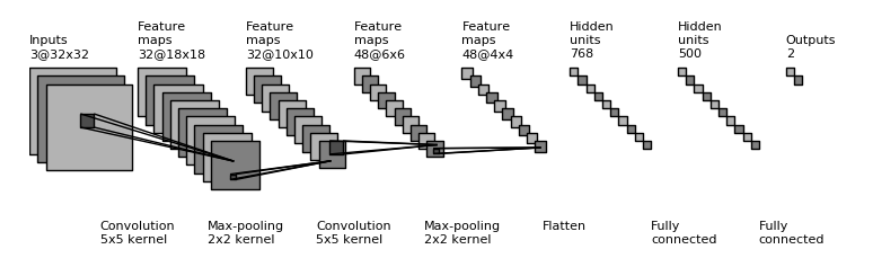
\includegraphics[width=300pt]{images/cnn/structure_CNN.png} 
\caption{Structure simplifiée d'un CNN. L'image est tirée de \cite{jefkine_backpropagation_2016} }
\label{structure_1}
\end{figure}

Ainsi, l'image en entrée est d'abord traitée par une succession de \textbf{couches de convolutions} suivies d'une \textbf{couche de pooling}. Ensuite ce processus se répète un certain nombre de fois et finalement le résultat passe par une ou plusieurs couches denses qui jouent le rôle d'un classifieur classique.

\subsection{Principe général}
Le principe directeur se cachant derrière les couches de convolution se base sur le fonctionnement même de notre vision : on dispose d'un noyau (\textit{kernel}) capable de reconnaître un motif en particulier. Il suffit alors de balayer l'image pixel par pixel (le balayage sera expliqué plus en détails ultérieurement) pour savoir où se trouvent précisément certains motifs sur l'image. En répétant ce procédé avec un grand nombre de noyaux différents, nous sommes capables de pouvoir identifier la présence ou non de certains motifs caractéristiques de l'objet à reconnaître. \\
Nous disposons ainsi d'une "carte" des différents motifs. Il nous est possible de la réduire en taille (étape de \textit{pooling}) pour réduire le nombre de calculs à effectuer. 
Le processus se répète un certain nombre de fois jusqu'à ce que l'on considère que les données soient suffisamment bien réduites pour qu'un MLP puisse s'en charger. 

\section{Formalisation d'un CNN}

\subsection{Le produit de convolution : un outil indispensable}

Le coeur de l'efficacité d'un CNN repose sur le produit de convolution. On assimile l'image à une matrice notée $I$ (nous la supposons pour l'instant en niveau de gris, de telle sorte que la matrice est en 2D mais la généralisation en 3D se fait aisément). De même, le noyau sera noté sous la forme d'une matrice $K$.
L'opération de convolution s'écrit alors : \\

$\forall (x,y) \in [0,W_I] \times [0,H_I] \, entiers \, $,  $(N \otimes I)_{x,y} = \sum_{i=0}^{W_K} \sum_{j=0}^{H_K} K_{i,j} \times I_{x-i,y-j}$ \\
\\
Où l'on a posé $W_I,H_I$ la taille de l'image et $W_K,H_K$ la taille du noyau. \\
\\
La figure \ref{chien_prairie} donne quelques exemples de l'effet du produit de convolution avec plusieurs noyaux.

\begin{figure}[!h]
\centering
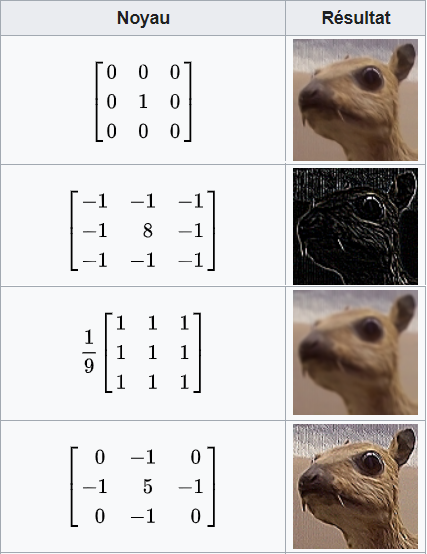
\includegraphics[width=150pt]{images/cnn/chien_prairie.png} 
\caption{Effets de la convolution avec quelques noyaux. L'image provient de Wikipedia.}
\label{chien_prairie}
\end{figure}

Ainsi, cette opération nous permet de mettre en évidence des motifs élémentaires en activant la case correspondante si le motif est présent au niveau de celle-ci.

\subsection{Le balayage de l'image : une histoire de Padding et de Stride}

Pour pouvoir évaluer toute l'image, il va falloir la balayer avec le noyau. De manière assez logique, on commence par se placer sur le coin supérieur gauche de l'image, puis on effectue un produit de convolution. Ensuite, il suffit de faire glisser latéralement le noyau d'un pixel et de répéter l'opération. Une fois au bout de la ligne, on descend d'un pixel et on repart à gauche. La figure \ref{convolution} donne un exemple de balayage d'un noyau sur une image.

\begin{figure}[!h]
\centering
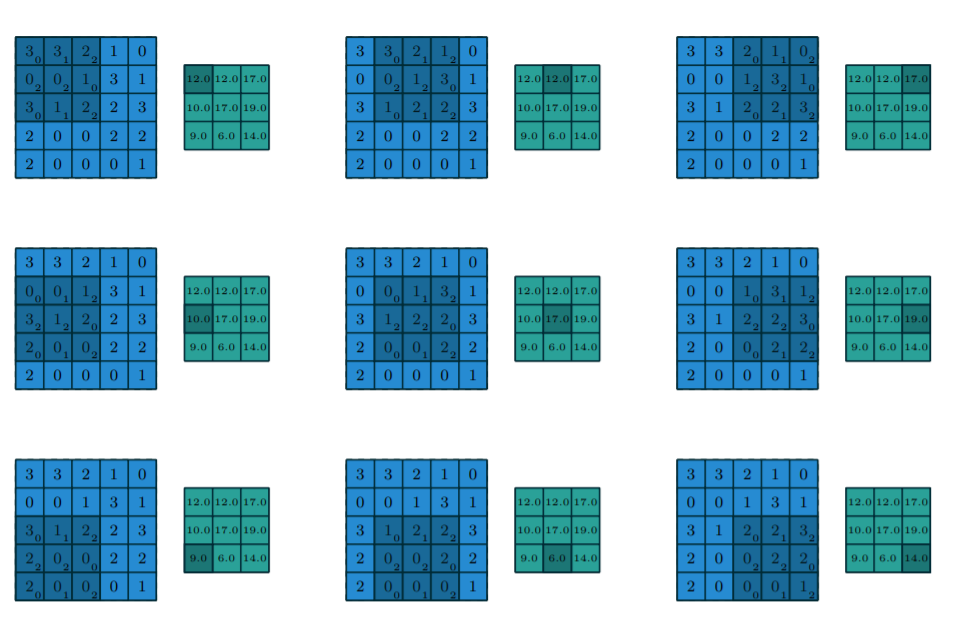
\includegraphics[width=200pt]{images/cnn/convolution.png}
\caption{Fonctionnement de la couche de convolution sur un exemple simple. L'image est tirée de l'article de Dumoulin et al. \cite{dumoulin_guide_2018}.}
\label{convolution}
\end{figure}

On remarque alors que le résultat a une dimension plus petite que l'image d'origine : on a ici effectué ce que l'on appelle un \textbf{simple padding}. Cependant, on pourrait souhaiter que le résultat ait la même dimension : cela est rendu possible grâce au \textbf{same padding}. Pour cela, nous pouvons rajouter des gardes autour de l'image d'origine : on rajoute des zéros autour puis on effectue l'opération de convolution comme présentée sur la figure \ref{same_padding}

\begin{figure}[!h]
\centering
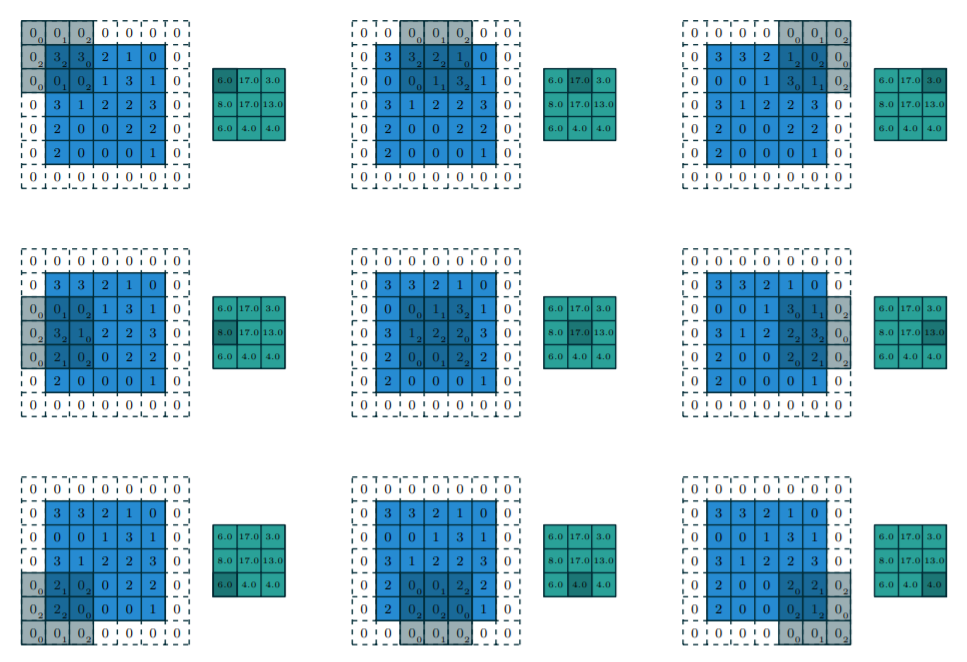
\includegraphics[width=200pt]{images/cnn/same_padding.png}
\caption{Fonctionnement de la couche de convolution avec du same padding. L'image est tirée de l'article de Dumoulin et al. \cite{dumoulin_guide_2018}.}
\label{same_padding}
\end{figure}

Il existe encore un paramètre permettant de personnaliser l'opération : le \textbf{stride}. Celui correspond au décalage à utiliser pour le noyau. Ce processus est représenté sur la figure \ref{stride}.

\begin{figure}[!h]
\centering
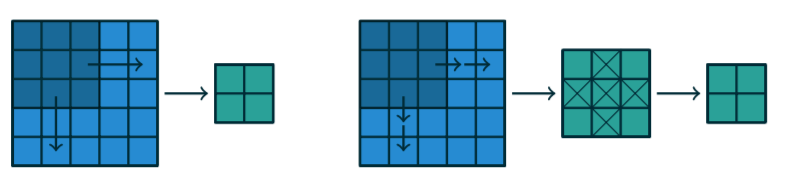
\includegraphics[width=200pt]{images/cnn/stride.png}
\caption{Fonctionnement de la couche de convolution avec un stride valant 2. À gauche, le résultat de l'opération. À droite, une façon différente de voir les choses : le noyau balaye toute la matrice avec un pas de 1 mais ne garde les valeurs que pour les déplacements pairs. L'image est tirée de l'article de Dumoulin et al. \cite{dumoulin_guide_2018}.}
\label{stride}
\end{figure}
 
L'avantage d'avoir un stride plus grand que 1 est aussi son désavantage : en effet il va permettre d'avoir un résultat en sortie de plus petite dimension mais en contrepartie, il provoque une perte d'information.

\subsection{Généralisation en 3D}

Les images en couleurs peuvent être représentées par une matrice 3D de profondeur 3. Pour pouvoir gérer ce cas, nous prenons des noyaux de la même profondeur que l'image, puis nous appliquons séparément le produit de convolution sur les profondeurs correspondantes, le résultat final n'étant que la somme des résultats sur chaque profondeur. Un exemple d'une telle opération est représenté par la figure \ref{CNN_3D}.

\begin{figure}[!h]
\centering
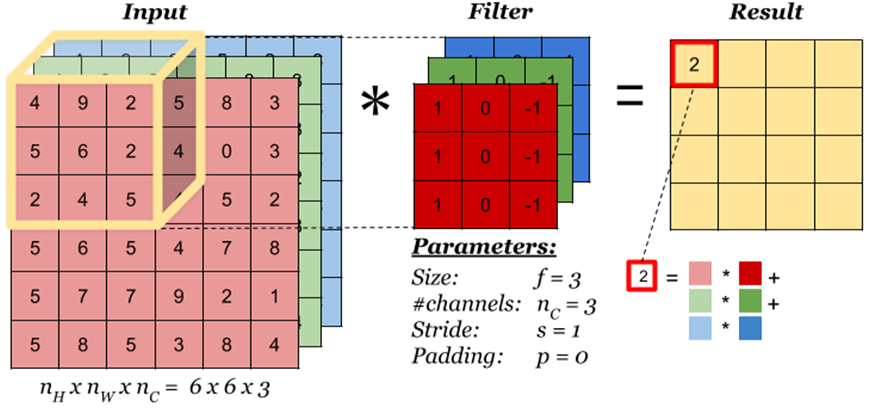
\includegraphics[width=200pt]{images/cnn/CNN_3D.png}
\caption{Exemple de convolution en 3D. L'image est tirée de l'article \textit{1D and 3D Convolution} de S.Verma \cite{verma_understanding_2020}.}
\label{CNN_3D}
\end{figure}

Notons cependant que ce résultat est très important car même si l'on considère que l'image n'a qu'une seule profondeur (image en niveau de gris par exemple), les données en entrée sur les autres couches de convolution sont dans l'immense majorité des cas en 3 dimensions. De manière intuitive, il est important de comprendre que la généralisation en 3D permet de détecter des motifs tridimensionnels au même titre qu'une opération de convolution simple permet d'identifier la présence d'un motif bidimensionnel. 

\subsection{Couche de pooling}

Les couches de pooling permettent de réduire la taille de la sortie au prix d'une perte d'information. Elles sont nécessaires pour compresser l'information. On considère généralement deux types de couches de pooling :

\begin{itemize}
 \item max pooling : on applique l'équivalent d'un noyau d'une opération de convolution qui ne retient que la valeur maximale de la zone sur laquelle il effectue les calculs. C'est la couche de pooling la plus utilisée. Un exemple de fonctionnement est présenté par la figure \ref{max_pooling}.
 
\begin{figure}[!h]
\centering
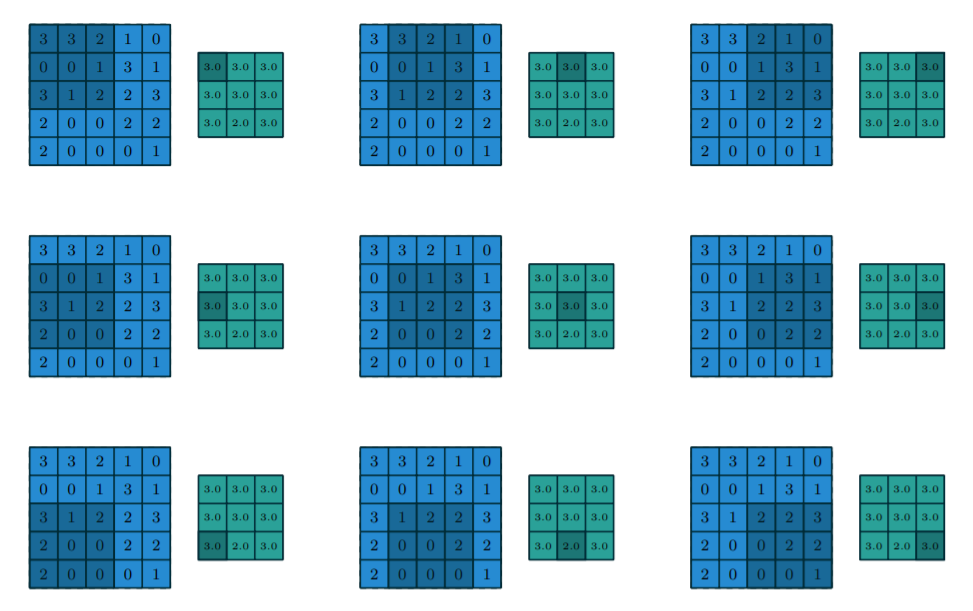
\includegraphics[width=200pt]{images/cnn/max_pooling.png}
\caption{Exemple simple d'application de la couche max pooling. L'image est tirée de l'article de Dumoulin et al. \cite{dumoulin_guide_2018}.}
\label{max_pooling}
\end{figure}
 
\item average pooling : le fonctionnement est le même que la couche de max pooling à sauf que l'on applique la fonction moyenne au lieu de la fonction maximum. Un exemple de fonctionnement est présenté par la figure \ref{avg_pooling}.
\end{itemize}

\begin{figure}[!h]
\centering
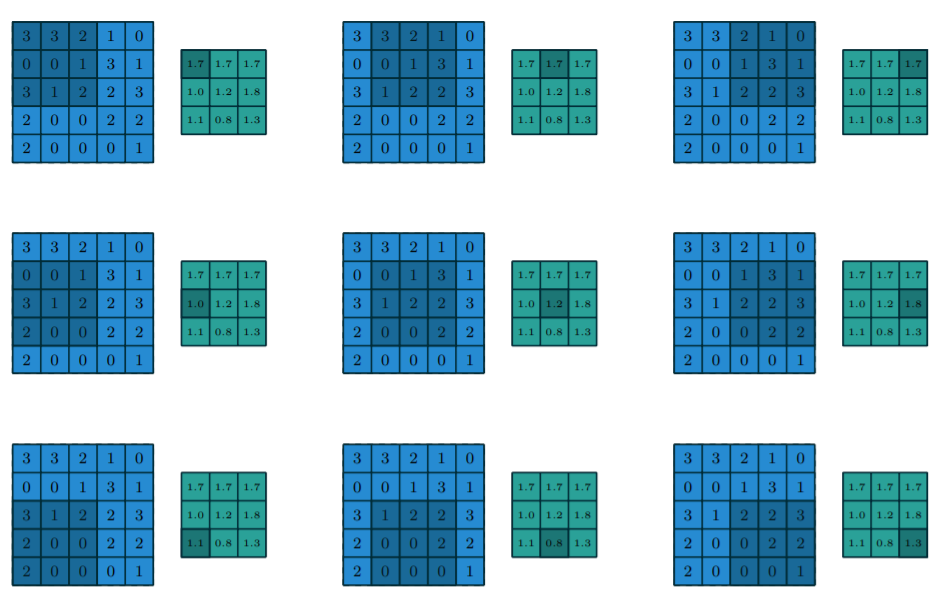
\includegraphics[width=200pt]{images/cnn/avg_pooling.png}
\caption{Exemple simple d'application de la couche avg pooling. L'image est tirée de l'article de Dumoulin et al. \cite{dumoulin_guide_2018}.}
\label{avg_pooling}
\end{figure}


Il est à noter que la taille des noyaux est une variable et que plus celle-ci est grande, plus la taille de la sortie sera petite. 
\subsection{Structure complète d'un CNN}

La reconnaissance d'objet est le plus souvent complexe et nécessite de nombreux motifs à déceler pour pouvoir être efficace. Ainsi, si l'on avait un motif par couche, la taille du CNN serait gigantesque. Pour éviter cela, il suffit d'associer à chaque couche plusieurs noyaux (généralement une puissance de 2). En appliquant les processus précédents pour chacun des noyaux, on se retrouve avec un nombre de matrice en sortie égal au nombre de noyaux. On se contente alors de les empiler en rajoutant une dimension supplémentaire. On obtient alors en sortie de couche de convolution, un bloc de profondeur égale au nombre de noyaux, contenant dans chacune des couches le résultat du produit de convolution pour un noyau. La figure \ref{structure_CNN_2} illustre ce principe.

\begin{figure}[!h]
\centering
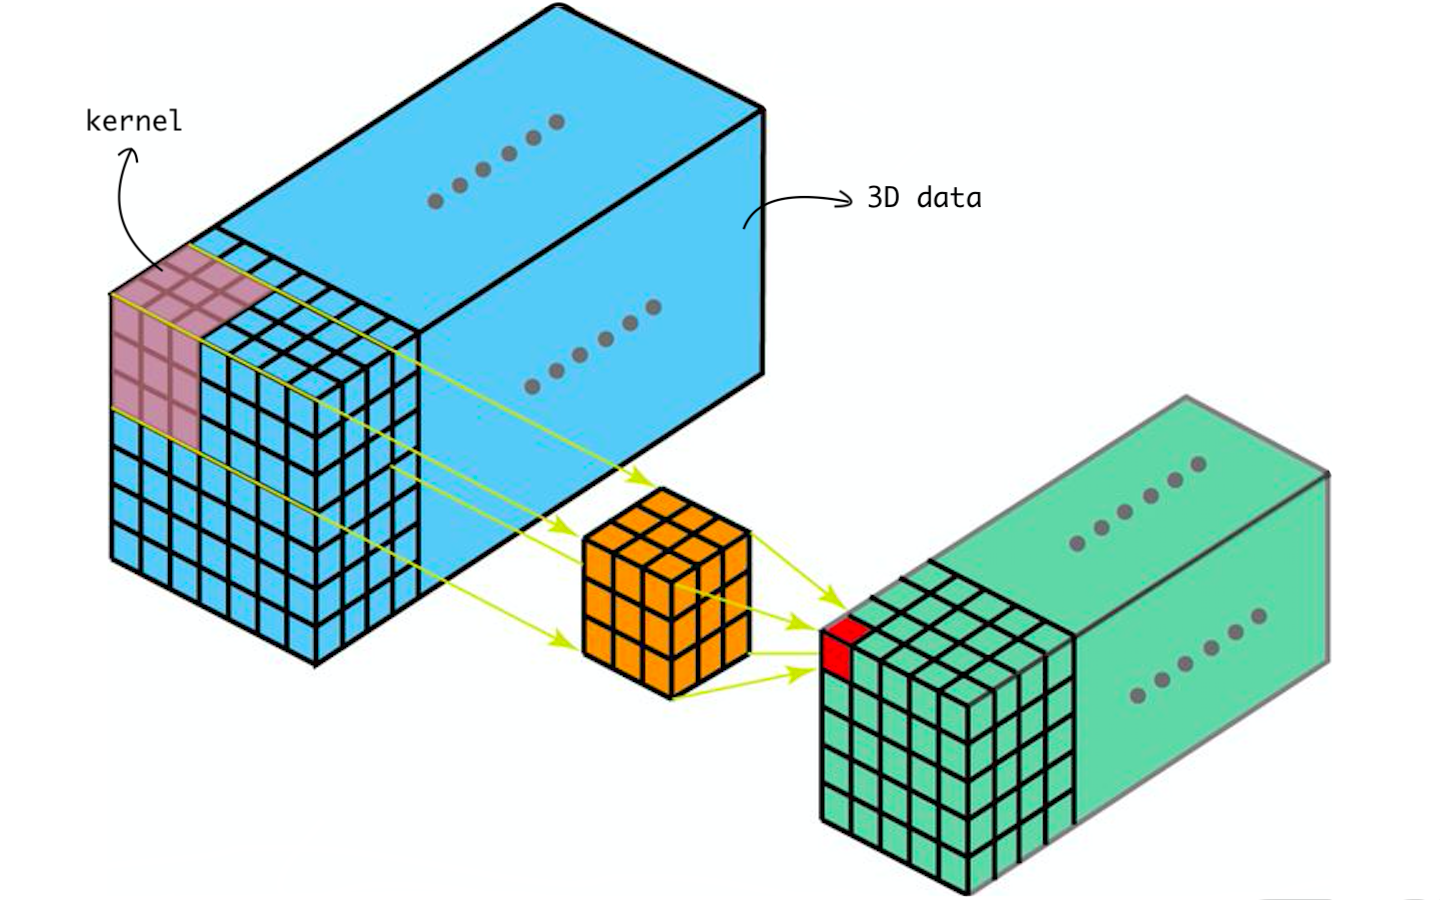
\includegraphics[width=200pt]{images/cnn/structure_CNN_2.png}
\caption{Exemple du résultat à la sortie d'une couche de convolution d'un CNN avec une structure complète. L'image est tirée de l'article \textit{1D and 3D Convolution} de S.Verma \cite{verma_understanding_2020}.}
\label{structure_CNN_2}
\end{figure}

On alterne ainsi entre couches de convolution pour prélever des motifs de plus en plus complexes et couches de pooling pour compresser les données. Les données étant ainsi pré-traitées, il suffit de les mettre en entrée d'une couche dense pour finalement avoir le résultat escompté.

\subsection{Apprentissage d'un CNN}

Le CNN, de par sa structure analogue à celle d'un MLP, a besoin d'une phase d'apprentissage dans le but d'apprendre à reconnaitre les motifs intéressants. Cela se fait par un processus de backpropagation. Cette partie étant essentiellement calculatoire, nous ne présenterons pas les opérations exactes à effectuer dans cette section. Les calculs sont essentiellement une généralisation de la rétropropagation présenté au chapitre 1. Pour plus d'informations, nous invitons le lecteur à consulter la littérature scientifique à ce sujet.
 
\subsection{Dropout}

Le principal problème de ce type d'architecture est le phénomène de sur-apprentissage. Pour pallier ce problème, des améliorations ont été proposées, notamment en 2014 par Srivastava et al. \cite{srivastava_dropout_nodate}. Les auteurs proposent en effet d'éteindre de manière aléatoire une certaine proportion de neurones (qui est un hyper-paramètre du dropout) pendant la phase de propagation avant (\textit{forward propagation}). Ils ont nommé cette technique le \textbf{dropout}. Cela permet de réduire la co-adaptation entre les neurones, évitant ainsi qu'un neurone ne prenne trop d'importance dans le processus d'apprentissage, ce qui pourrait amener à du sur-apprentissage. Une explication visuelle est proposée par la figure \ref{dropout}.

\begin{figure}[!h]
\centering
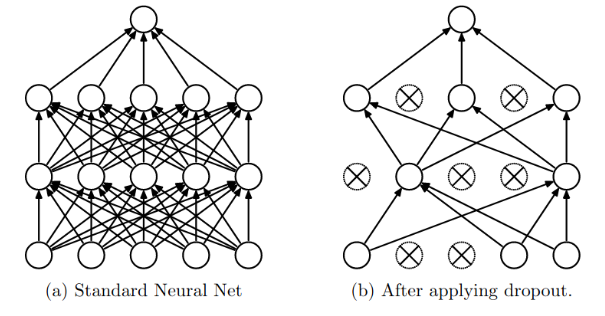
\includegraphics[width=300pt]{images/cnn/dropout.png}
\caption{A gauche, une structure MLP classique. A droite, un exemple de l'effet du dropout(paramètre ajusté à 50\%). Cette image vient de l'article de Srivastava et al. \cite{srivastava_dropout_nodate}.}
\label{dropout}
\end{figure}

La figure \ref{dropout_article} présente les résultats de ce même article. Les résultats sont plus que positifs dans la mesure où la qualité prédictive du réseau est grandement améliorée par le dropout.

\begin{figure}[!h]
\centering
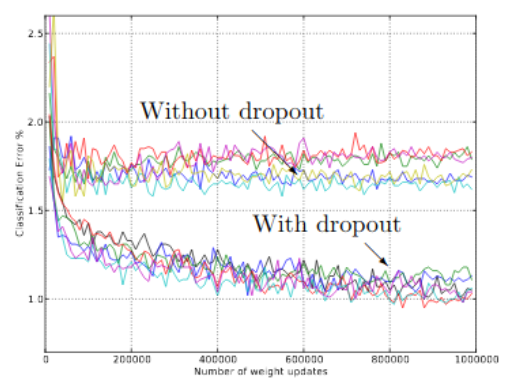
\includegraphics[width=200pt]{images/cnn/dropout_article.png}
\caption{Résultats de l'article sur l'efficacité du dropout sur un réseau neuronal. Cette image vient de l'article de Srivastava et al. \cite{srivastava_dropout_nodate}.}
\label{dropout_article}
\end{figure}
 
\section{Implémentation et résultats}

\subsection{Implémentation}

Nous avons une nouvelle fois utilisé TensorFlow 2.0 qui permet l'utilisation rapide de couches telles que celles de convolution, de pooling mais aussi de \textit{flatenning}. La couche de \textit{flatenning} est une couche permettant de faire la transition entre la dernière couche de convolution et la première couche dense. En d'autres termes, elle transforme les données en 3 dimensions en un tableau en 1 dimension.\\
La structure du réseau simplifié avec lequel nous avons fait les tests est la suivante :

\[ \begin{array}{lcr}
	Conv2D(64, 3, activation=relu) \\
    Conv2D(32, 3, activation=relu) \\
    Flatten() \\
    Dense(128, activation=relu) \\
    Dense(10, activation=softmax)\end{array}\]

Nous avons de plus utilisé l'optimiseur ADAM pour effectuer la descente de gradient.

\subsection{Résultats}

Nous avons tout d'abord voulu tester la taille des noyaux pour voir quelle influence celle-ci a sur les performances de notre CNN. La figure \ref{resultat_noyaux} présente les résultats sur la base de données MNIST.

\begin{figure}[!h]
\centering
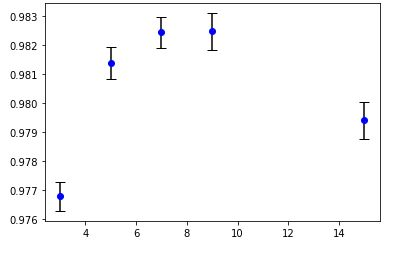
\includegraphics[width=200pt]{images/cnn/resultat_noyau.png}
\caption{Comparaison de la précision de notre CNN en fonction de la taille des noyaux. En ordonnée la précision, en abscisse la taille des noyaux. La base de données utilisée est MNIST.}
\label{resultat_noyaux}
\end{figure}

Nous pouvons en déduire que des noyaux de taille trop grande par rapport aux images d'origine risquent de nuire à l'efficacité du CNN. \\

Nous nous sommes, de plus, intéressés à l'influence du \textbf{stride} et du \textbf{padding} sur les performances du CNN. La figure \ref{resultat_padding_stride} présente les résultats de notre analyse sur MNIST.

\begin{figure}[!h]
\centering
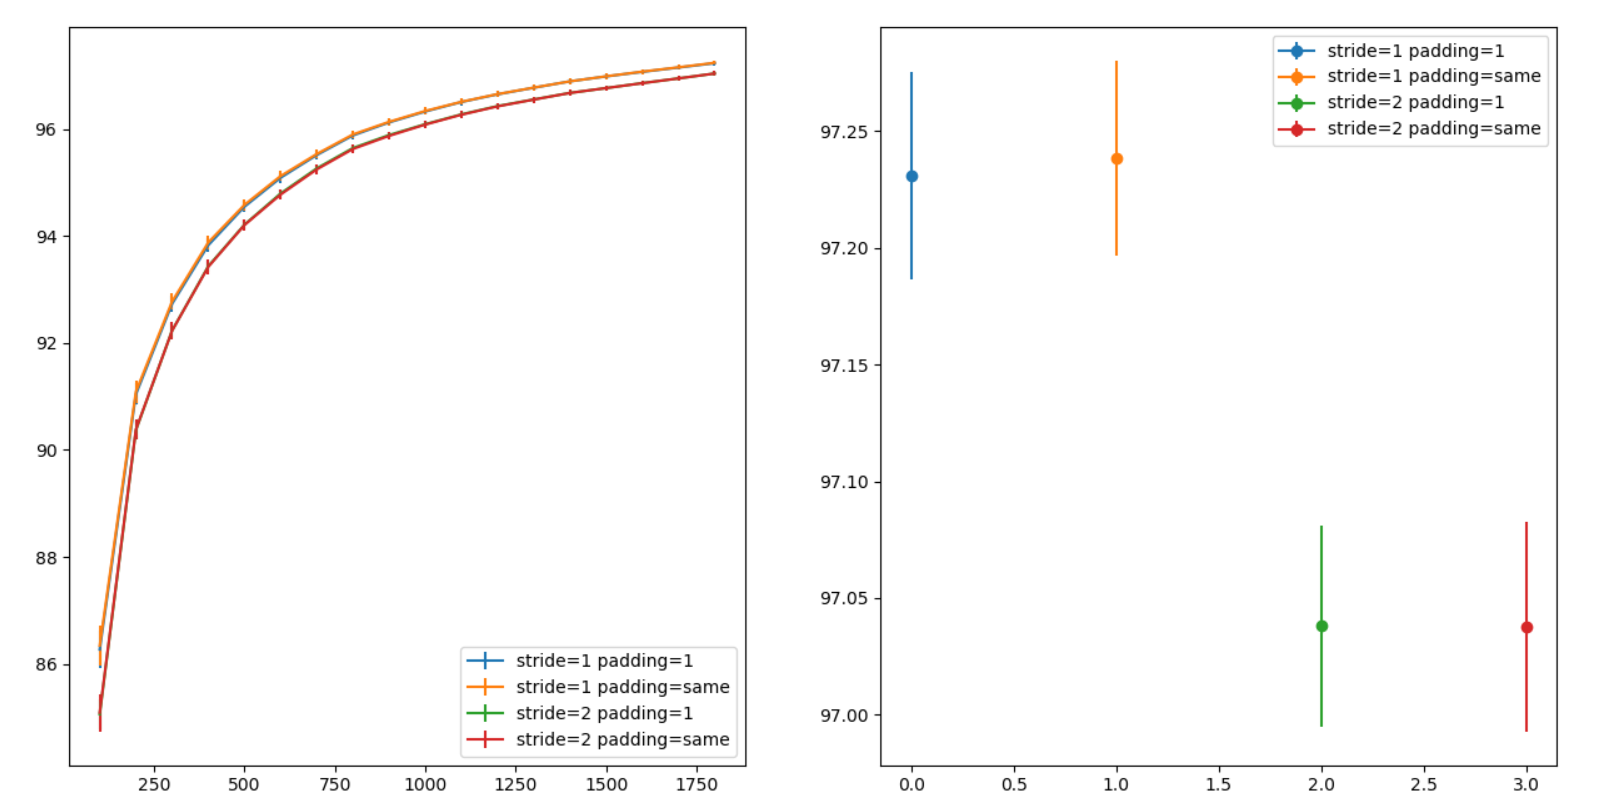
\includegraphics[width=300pt]{images/cnn/CNN_padding_stride.png}
\caption{Comparaison de la précision de notre CNN en fonction des paramètres stride et padding. En ordonnée la précision, en abscisse le nombre de batchs d’entraînement. La base de données utilisée est MNIST.}
\label{resultat_padding_stride}
\end{figure}

Nous pouvons conclure que, sur cette base de données, l'utilisation d'un stride supérieur à 1 a comme effet de réduire les capacités prédictives du CNN. En effet, lorsque ce paramètre est trop élevé, la perte d'information est trop importante, nuisant aux performances de l'algorithme. Nous remarquons de plus que le padding n'a ici aucune influence. Ce résultat n'est pas surprenant car les images de MNIST sont centrées avec des bords sombres. Ainsi il n'y a aucune information sur les bords, rendant le changement de padding quasiment inutile. \\

De même, nous avons testé l'influence du \textbf{dropout}. Les résultats sont présentés sur la figure \ref{resultat_dropout}. Les résultats sont beaucoup moins significatifs que ce que laisse présager l'article de Srivastava et al. \cite{srivastava_dropout_nodate}. Il semble donc que le dropout n'a aucune influence sur les résultats de notre CNN. Ceci est probablement dû à la banque d'images MNIST et à la petite taille de notre réseau, qui ne sont pas propices au sur-apprentissage .
  
\begin{figure}[!ht]
\centering
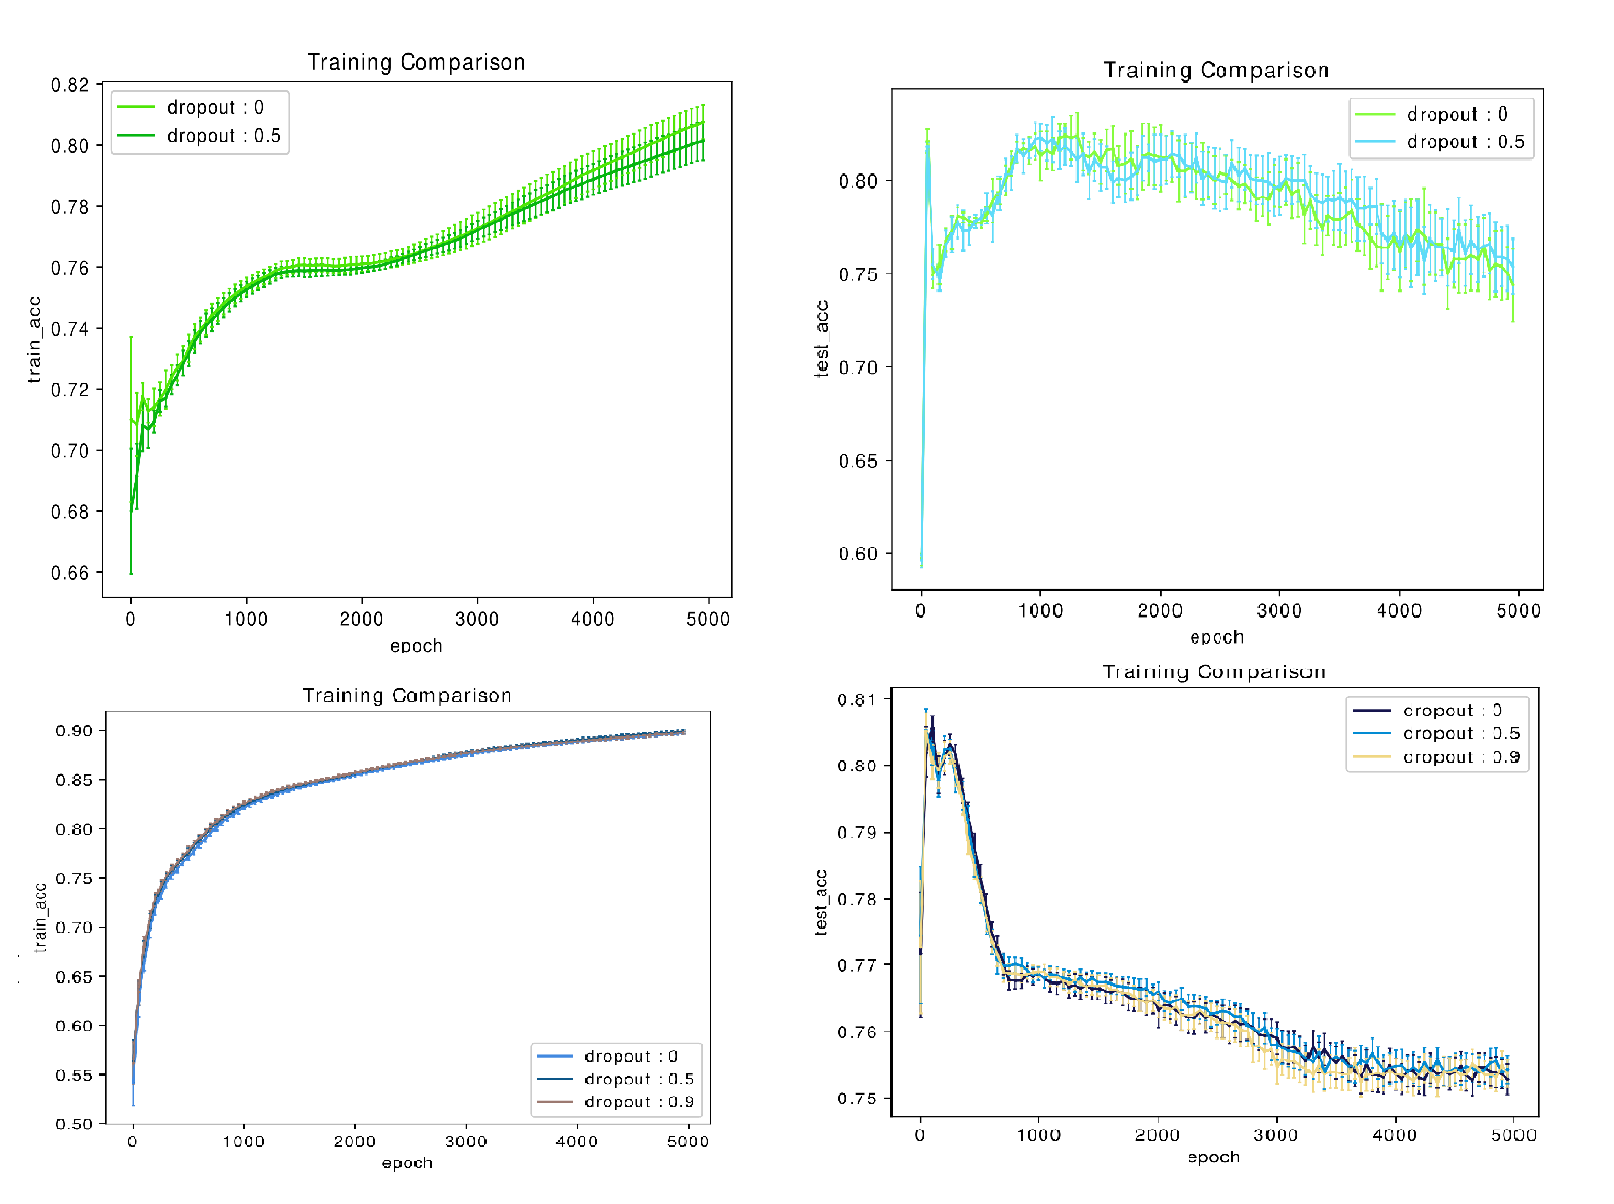
\includegraphics[width=340pt]{images/cnn/resultat_dropout.png}
\caption{Influence du dropout sur l'efficacité de nos réseaux. En haut, un CNN sur la base de données MNIST. En bas, un MLP sur la base de données Moon. Nous remarquons que les courbes sont toutes confondues, quel que soit le paramètre de dropout choisi.}
\label{resultat_dropout}
\end{figure}

\section{Conclusion}

Ainsi, le CNN s'avère être une formidable avancée dans la détection de motifs par rapport au classique multiperceptron. En effet, celui-ci opère un traitement de l'image beaucoup plus fin grâce à la technologie des couches convolutives. Cela lui permet entre autre d'avoir une vision plus globale de l'image et de pouvoir extraire plus facilement des motifs récurrents. Comme nous souhaitons travailler sur de la génération d'image, il nous a été indispensable de maîtriser et de comprendre en profondeur le fonctionnement de cette structure algorithmique. 

 




\chapter{Les GAN (Réseaux Adverses Génératifs)}

\section{Principe général des GAN}
Le principe général des GAN repose sur l'utilisation de deux réseaux, ayant des objectifs contraires, on dit qu'ils sont \textbf{adversaires}. Le premier réseau transforme du bruit en image, c'est le \textbf{générateur} (G). Le deuxième réseau prend en entrées des images et les classe en deux catégories, en leur associant leur probabilité d'être issues de la base de donnée : c'est donc un classifieur binaire, il est appelé \textbf{discriminateur} (D). Le plus souvent, le discriminateur sera alimenté par des images de deux sortes : celles provenant de la base de donnée (images réelles), et celles générée par le générateur, son rôle sera donc de dire si une image est réelle ou générée. Il s'agit ensuite d'entraîner G afin qu'il maximise la probabilité que D fasse une erreur, et d'optimiser D afin qu'il améliore la justesse de sa classification.

L'architecture des GAN a été introduite pour la première fois par Ian Goodfellow \cite{goodfellow_generative_2014} en 2014. Cet article innovant montrait déjà un gain de performance pour la génération d'images suivant une base de donnée. Mais l'atout majeur des GAN sont leur adaptabilité à tous types de données.


\section{Le DCGAN (Deep Convolutionnal Adversarial Network)}
Le DCGAN utilise la fonction de coût proposée par Goodfellow \cite{goodfellow_generative_2014}, mais le générateur et le discriminateur sont tous les deux des \textbf{réseaux à convolutions} \cite{radford_unsupervised_2015-1}. La fonction de coût de G à minimiser est la suivante : $$\begin{aligned}
\mathcal{L}_{\mathrm{DCGAN}}\left(G, D, p_{\mathrm{data}}, p_{\mathrm{bruit}}\right) &=
   \mathbb{E}_{x \sim p_{\mathrm{data}}}(\log (D(x))) + \mathbb{E}_{z \sim \mathrm{p_{bruit}}}(\log (1 - D(G(z)))
\end{aligned}$$

Pareillement, on donne comme fonction de coût pour D l'opposé de celle de G. L'architecture du DCGAN correspond alors à un jeu à somme nulle. La théorie des équilibres de Nash donne un unique état stable. Il correspond à un coût égal à $-\log 4$ pour G et $ \log 4$ pour D. Dans cette configuration, le discriminateur est forcé d'associer une probabilité de 0,5 pour chaque image donnée en entrée, le générateur étant devenu trop fort.

Une variation intéressante sur le DCGAN est de poser $  \mathbb{E}_{x \sim p_{\mathrm{data}}}(\log (D(x))) + \mathbb{E}_{z \sim \mathrm{bruit}}(\log (D(G(z)))$ comme fonction de coût en début d'apprentissage. L'intérêt de cette modification résulte d'un problème : le discrimateur a tendance à facilement distinguer les images générées par G de celles de la base de donnée en début d'apprentissage. Dans ce cas, le terme $\log (1 - D(G(z))$ sature vers 0. Le remplacer par $\log (1 - D(G(z))$ résoud ce problème.


\section{Étude de la convergence des GAN}

De par leur caractère d'adversaires, les GAN requièrent un équilibre fin entre la générateur et le discriminateur, ils sont donc par nature \textbf{instables}. L'étude de la convergence des GAN est un domaine encore très actif de la recherche. Nous allons discuter de deux phénomènes très communs qui peuvent gêner ou ruiner l'apprentissage des GAN : l'\textbf{effondrement des modes} (\textit{mode collapse}), et la \textbf{non-convergence} due à la perte d'équilibre du système.

\subsection{L'effondrement des modes}

\begin{figure}[!h]
\centering
\includegraphics[width=100pt]{"images/GAN/collapseA_1"}
\includegraphics[width=100pt]{"images/GAN/collapseA_2"}
\caption{Exemples d’effondrement des modes sur la banque de chiffres MNIST.}
\label{mode_collapse}
\includegraphics[width=100pt]{"images/GAN/collapseB_1"}
\includegraphics[width=100pt]{"images/GAN/collapseB_2"}
\caption{À gauche, un exemple d'effondrement des modes sur la banque d'image CelebA. À droite, une génération sans effondrement pour comparaison. On observe que sur l'image de gauche, tous les personnages ont la même tête.}
\label{mode_collapse_celeb}
\end{figure}


L'effondrement des modes survient quand le réseau générateur ne génère pas des images conforment à l'ensemble de la distribution des images réelles, mais seulement à une petite partie. L'effondrement des modes est très visible lorsque la distribution des images réelles forme des zones bien séparées, c'est à dire quand celle-ci comporte des classes bien définies. La manifestation de ce phénomène se traduit par des images générées qui se ressemblent toutes. Les figures \ref{mode_collapse} et \ref{mode_collapse_celeb} montrent des exemples du phénomène sur la base de données MNIST et CelebA.


Pour mieux comprendre le phénomène, il est intéressant de regarder la distribution des images de MNIST dans son ensemble. Cela est possible grâce à des algorithmes de réduction de dimension. Attention, la réduction de dimension se fait dans l'espace des pixels, et non pas dans un espace sémantique, la visualisation ne permet donc pas de séparer efficacement les différentes classes, elle permet seulement un aperçu de la distribution dans l'espace sémantique. Les figures \ref{tsne1} et \ref{tsne2} présentent une visualisation de MNIST par transformation t-SNE \cite{van_der_maaten_visualizing_2008}.

\begin{figure}[!h]
\centering
\includegraphics[height=90pt]{"images/GAN/modes1"}
\includegraphics[height=90pt]{"images/GAN/modes1_tsne"}
\caption{On observe un effondrement à deux modes. Le GAN ne génère que des un et des huit, correspondant aux point rouges sur la représentation t-SNE}
\label{tsne1}
\includegraphics[height=90pt]{"images/GAN/modes2"}
\includegraphics[height=90pt]{"images/GAN/modes2_tsne"}
\caption{On observe un effondrement à un mode. Le GAN génère un symbole non présent dans la base MNIST. Sur la représentation t-SNE, les points rouges ne correspondent à aucun nuage de points}
\label{tsne2}
\end{figure}

L'ensemble de points rouges correspond à un ensemble d'images générées par le réseau générateur lors de l'effondrement des modes. Sur les données MNIST, on observe différents groupes de points (des \textit{clusters}), ce sont les \textbf{modes} inhérents à la base de donnée MNIST : les chiffres de 1 à 9. Ce qu'il est intéressant de noter, c'est que les points générés sont rassemblés autour de un ou plusieurs pôles denses très localisés, qui ne sont pas répartis dans tout l'espace. Cela traduit l'effondrement des modes : les images générées ne couvrent qu'une petit partie de la distribution de la base de donnée d’entraînement.\\

Il n'y a pas de solution simple, directe et universelle pour lutter contre l'effondrement des modes, mais quelques solutions ont été proposées :
\begin{itemize}
  \item La pénalisation de la similarité des images en sortie de générateur \textit{minibatch discrimination}. Cela consiste à ajouter un terme à la fonction de coût pour traduire la similarité (il peut s'agir de calculer une similaire pixel à pixel, ou d'estimer la similarité sémantique avec un autre réseau de neurones).
  \item Le \textit{one-side label smoothing}. Cela consiste à changer l'objectif du discriminateur : son objectif ne sera plus de discriminer les fausses images avec une probabilité de 1, mais une probabilité plus faible, par exemple 0.9. Cela permet d'éviter la sur-confiance, et permet de laisser le générateur explorer tous l'espace des images réelles.
  \item Certaines architectures sont plus résistantes que d'autres à l'effondrement des modes. Par exemple, les GAN de Wasserstein [\ref{WGAN}] ne présentent ce problème. 
\end{itemize}


\subsection{Perte de l'équilibre}

Comme expliqué plus haut, l'apprentissage des GAN repose sur un équilibre fin entre le discriminateur et le générateur. Cet équilibre est parfois difficile à atteindre et est souvent instable, c'est pourquoi parfois le système s'effondre complètement. Cet effondrement vient souvent du fait que le discriminateur est devenu "trop fort" (sa fonction de perte tombe à zéro), et le générateur ne peut plus s'améliorer. Lorsque cela arrive, l’entraînement peut être arrêté : les images générées ne s'amélioreront plus. Un exemple de ce phénomène et illustré dans la figure \ref{perte_eq}, où l'on voit qu'à partir d'un cycle d’entraînement, la fonction de perte du discriminateur s'écroule et celle du générateur diverge.

\begin{figure}[!h]
\centering

\includegraphics[width=130pt]{"images/GAN/failure3"}
\caption{L'erreur du discriminateur - en orange - devient rapidement quasiment nulle, tandis que celle du générateur - en bleu - explose}
\label{perte_eq}
\end{figure}


Il existe des solutions pour lutter contre ce problème, et cela consiste souvent à rééquilibrer les puissances ou les vitesse de convergence des différents réseaux. On peut par exemple diminuer la complexité du discriminateur, diminuer le taux d'apprentissage du discriminateur, ou mettre à jouer plus souvent le générateur que le discriminateur.
Ajouter du bruit sur les images de la base de donnée permet aussi se renforcer la stabilité de l'apprentissage. Par ailleurs, on peut noter que les GAN de Wassertein sont plus stables que les DCGAN, mais ne sont pas totalement immunisés aux problèmes de convergence.

\section{Cadre théorique et WGAN}
Nous allons essayer dans cette section de donner un cadre probabiliste et statistique rigoureux permettant d'expliquer le fonctionnement des GAN. Cette approche permettra de justifier l'algorithme WGAN qui permet de significativement réduire les problèmes d'apprentissage des GAN.

\subsection{Approche bayésienne des GAN}
L'objectif d'un GAN - la génération d'images suivant un dataset - peut être formalisé comme un problème d'optimisation bayésienne. Nous cherchons à approcher la distribution $p_{\mathrm{data}}$ d'une variable aléatoire $X: \Omega \longrightarrow \mathcal{X}$. Pour ce faire, on se donne une famille paramétrique de distributions $\mathcal{M}_{\mathbb{R}^{d}} = \{p_{\theta}, \theta \in \mathbb{R}^d\}$, ainsi qu'un prior $p_{\mathrm{bruit}}(z)$ relatif à une variable aléatoie $Z : \Omega \longrightarrow \mathcal{Z}$. On détermine ensuite la distribution souhaitée à l'aide de la formule de Bayes. $$\begin{aligned} p(\theta | \mathrm{data}) \propto p_{\mathrm{bruit}}(z)p(\mathrm{data}|\theta)\end{aligned}$$

Comme il est impossible de résoudre directement la formule de Bayes, il nous faut défnir une fonction de côut qui mesure la distance entre $p_{\theta}$ et $p_{\mathrm{data}}$, puis employer des algorithmes de descente du gradient. La famille $\mathcal{M}_{\mathbb{R}^d}$ prend alors naturellement la forme d'un réseau de neurones, que l'on écrit $g : \mathcal{Z} \times \mathbb{R}^{d} \longrightarrow \mathcal{X}$, ou en notation condensée $g_{\theta}(z)$ .

\subsection{DCGAN} \label{DCGAN_prob}

Le DCGAN utilise la métrique $\delta$ pour mesurer l'écart entre deux distributions $p_{\mathrm data}$ et $p_{\theta}$, définie par la relation suivante. 

$$\begin{aligned} \delta(p_{\mathrm{data}}, p_{\theta}) = -\log 4 + 2 \mathrm{DJS}(p_{\mathrm{data}} || p_{\theta})\end{aligned}$$ où DJS est la divergence de Jensen-Shanon.

On peut montrer \cite{goodfellow_generative_2014} la relation suivante, en posant $\mathcal{F}$ l'ensemble des fonctions continues $\mathcal{X} \longrightarrow (0,1)$.

$$\begin{aligned} \delta(p_{\mathrm{data}}, p_{\theta}) = \sup_{f\in\mathcal{F}} \mathbb{E}_{x \sim p_{\mathrm{data}}}(\log (f(x))) + \mathbb{E}_{x \sim p_{\theta}}(\log (1 - f(x)))\end{aligned}$$

On remarque alors si $f: \mathcal{X} \longrightarrow (0,1)$ est solution de ce problème on peut calculer $\nabla_{\theta} \delta$, dans l'optique d'optimiser $g_{\theta}(z)$. 

$$\begin{aligned}\nabla_{\theta} \delta(p_{\mathrm{data}}, p_{\theta}) = \mathbb{E}_{z\sim p_{\mathrm{bruit}}(z)} \left( \frac{\nabla_{\theta}f(g_{\theta}(z))}{f(g_{\theta}(z)) -1} \right)\end{aligned}$$.

Il nous reste encore à déterminer $f$. Il est intuitif de chercher à calculer $f$ comme un réseau de neurones $\{f_{w}, w \in \mathcal{W} \}$, qui peut être optimisé par rétropropagation à partir de  $\mathbb{E}_{x \sim p_{\mathrm{data}}}\left(\frac{\nabla_{w}f_{w}(x)}{f_{w}(x)}\right)+ \mathbb{E}_{z \sim p_{\mathrm{bruit}}}\left(\frac{\nabla_{\theta}f(g_{\theta}(z))}{f(g_{\theta}(z)) -1}\right)$.

Ce formalisme nous renvoie donc à la définition du DCGAN par sa fonction de coût pour G (ici $g_{\theta}$) et D (ici $f_{w}$). En effet, on a la relation suivante : 

$$\begin{aligned}
\delta(p_{\mathrm{data}}, p_{\theta}) = \sup_{f\in\mathcal{F}} \mathcal{L}_{\mathrm{DCGAN}}(g_{\theta}, f, p_{\mathrm{data}},  p_{\mathrm{bruit}})
\end{aligned}$$

\subsection{WGAN} \label{WGAN}

Les Wasserstein GAN, ou WGAN, on été introduits en 2017 par Arjovsky et al. \cite{arjovsky_wasserstein_2017}. Les auteurs y introduise une nouvelle distance, la distance 1-Wasserstein (qu'on appelera ici distance Wassertein), définie par la relation suivante:

$$\begin{aligned}
W(p_{\mathrm{data}}, p_{\theta}) = \inf_{\gamma \in \Pi (p_{\mathrm{data}}, p_{\theta})} \mathbb{E}_{(x, y) \sim \gamma} (||x - y||)
\end{aligned}$$
Avec $\Pi (p_{\mathrm{data}}, p_{\theta})$ l'ensemble des densité de distributions jointes $\gamma (x, y)$ de lois marginales respectivement $p_{\mathrm{data}}$ et $p_{\theta}$. On peut réecrire ce résultat à l'aide de la formulation duale du théorème de Kantorovich \cite{villani_optimal_2006}.


$$\begin{aligned}
W(p_{\mathrm{data}}, p_{\theta}) = \sup_{f \in L_{1}}\left(\mathbb{E}_{x\sim p_{\mathrm{data}}} [f(x)] - \mathbb{E}_{x\sim p_{\theta}} [f(x)]\right)
\end{aligned}$$
 Avec $L_{1}$ l'ensemble des fonctions 1-lipschitziennes $\mathcal{X} \longrightarrow \mathbb{R}$. On obtient donc une équation assez similaire à celle du paragraphe \ref{DCGAN_prob}. Nous allons estimer $f$ par un réseau de neurones $\{f_{w}, w \in \mathcal{W} \}$ qui sera optimisé à l'aide du gradient $\mathbb{E}_{x\sim p_{\mathrm{data}}} \left[\nabla_{w}f_{w}(x)\right] - \mathbb{E}_{z\sim p_{\mathrm{bruit}}} \left[\nabla_{w}f_{w}(g_{\theta}(z))\right]$. De même, à $f$ fixé, $g_{\theta}(z)$ s'optimise par rétropagation du gradient selon $\theta$.
 
\subsection{Avantages comparatif du WGAN par rapport au DCGAN}
 
Maintenant que nous savons ce qu'est un WGAN, il s'agit de comprendre son avantage par rapport au DCGAN. D'abord, la distance $W$ est topologiquement plus faible que la divergence de Jensen-Shanon, et donc par extension que $\delta$. Ceci signifie qu'il est plus facile en pratique de faire converger un WGAN qu'un DCGAN.

Ensuite, à chaque boucle d'apprentissage, le WGAN peut mieux optimiser le discriminateur avant de faire apprendre le générateur. En effet, pour un WGAN, meilleur est le discriminateur, meilleur est le gradient utilisé pour l'apprentissage du générateur. Ceci permet de résoudre le problème d'instabilité au début de l'apprentissage rencontré dans les DCGAN, pour lesquels un discriminateur trop bon fait saturer le gradient du générateur à 0.

Finalement, la capacité du WGAN d'entraîner d'abord le discrimnateur empêche le phénomène du mode collapse. En effet, la cause du mode collapse est que pour un discriminateur fixé, le meilleur générateur est celui qui ne génère que les points de $\mathcal{X}$ de plus grande valeur pour le discriminateur.

\section{Implémentation et résultats}

Nous avons implémenté avec succès l'algorithme WGAN pour la base de donnée MNIST, et  DCGAN pour les banques de données MNIST et CelebA. 

\subsection{Détails de l'implémentation}

Nous avons utilisé la même structure de réseau pour le DCGAN et le WGAN, en changeant uniquement la fonction de coût.


\textbf{Pour le discriminateur},
\[ \begin{array}{lcr}
Conv2D(64, (5,5), strides=(2,2)) \\
LeakyReLU() \\
Dropout\\

Conv2D(128, (5,5), strides=(2,2)) \\
BatchNormalization\\
LeakyReLU()\\
Dropout\\

Conv2D(256, (5,5), strides=(2,2)) \\
BatchNormalization\\
LeakyReLU()\\
Dropout\\


Flatten()\\
Dense(1)\\
LeakyReLU()\\

\end{array}\]

\textbf{Pour le générateur,} 

\[ \begin{array}{lcr}
Dense(240)\\
LeakyRelu()\\
Reshape((10, 8, 3))\\

Conv2DTranspose(256, (5,5), strides=(2,2)) \\
BatchNormalization\\
LeakyReLU() \\


Conv2DTranspose(64, (5,5), strides=(2,2)) \\
BatchNormalization\\
LeakyReLU() \\

Conv2DTranspose(3, (5,5), strides=(2,2)) \\

\end{array}\]

\subsection{MNIST}

Nous présentons ici les résultats obtenus après 50 passes sur la base de données MNIST, à l'aide des algorihtmes DCGAN et WGAN. On observe que nous avons eu plus de mal dans l'implémentation du WGAN, et n'arrivons pas à obtenir le gain de performance prédit par l'article \cite{arjovsky_wasserstein_2017}.

\begin{figure}[!h]
\centering
\includegraphics[width=100pt]{"images/GAN/MNIST_DCGAN"}
\includegraphics[width=100pt]{"images/GAN/MNIST_WGAN"}
\caption{A gauche, 16 images générées par le DCGAN. A droite, 16 images générées par le WGAN}
\label{mnist_gan}
\end{figure}

\subsection{CelebA}

Nous présentons ici les résultats obtenus après 400 passes sur la base de données CelebA. Nous avons donc réussi à construire avec succès un générateur de visages réalistes sans mode collapse.

\begin{figure}[!h]
\centering
\includegraphics[width=300pt]{"images/GAN/DCGAN"}
\caption{39 images obtenues par DCGAN sur la base CelebA}
\label{celeb_gan}
\end{figure}

\section{Conclusion}

Les GAN sont donc une technologie puissante de génération de données suivant une ditribution. S'affranchissant de la nécessité d'optimiser une famille de distributions paramétriques en maximisant la vraisemblance, ils permettent une généralisation sans précédent. Couplés avec des réseaux à convolutions, spécialisés dans le traitement des images, nous obtenons des résultats remarquables en génération d'images. Plus particulièrement, nous avons implémenté avec succès un algorithme DCGAN pour la génération de visages. Connaissant la précison avec laquelle le cerveau humain discerne les visages, il est surprenant d'en générer qui nous paraissent vraisemblables.
\chapter{Le cycleGAN}

\section{Présentation de la problématique}


Les cycleGAN, proposées par Zhu et al. \cite{zhu_unpaired_2018}, sont des architectures dérivées des GAN qui permettent de répondre à une problématique bien spécifique : le \textbf{transfert de style non appairé} \cite{gatys_image_2016}. Pour comprendre l’intérêt du cycleGAN, il faut bien comprendre le problème auquel il répond.
Le transfert de style consiste à transformer des données d'un \textit{style à un autre}. Le terme de \textit{style} est à prendre au sens large et les données que l'on manipule peuvent être de natures diverses. Il peut s'agir par exemple de transformer des images de pommes en images d'oranges, de transformer un paysage d'été en un paysage d'hiver, de transformer une musique classique en musique rock, ou encore de modifier les expressions faciales d'individus présents sur une image. Quelques exemples sont présentés sur la figure \ref{cycle_exemples}.

\begin{figure}[!h]
\centering
\includegraphics[width=200pt,valign=t]{"images/cycle/cycle_exemples"}
\caption{Exemples de transfert de style effectués par un cycleGAN. De haut en bas : transformation $pommes \leftrightarrow oranges$, transformation $paysages \, d'\acute{e} t \acute{e} \leftrightarrow paysages\,d'hiver$ et transformation $chevaux \leftrightarrow z\grave{e}bres$. Ces exemples sont tirés de l'article de Zhu et al. \cite{zhu_unpaired_2018}.}
\label{cycle_exemples}
\end{figure}


Le transfert de style peut se faire entre deux \textit{classes de styles} ou plus, mais nous allons ici nous concentrer sur le cas binaire, où l'on considère deux styles. La problématique est donc de transformer des images d'un style à l'autre, et ceci dans les deux sens.

Le transfert de style (à deux classes) repose sur deux banques de données que l'on notera ici A et B, et par extension nous parlerons du style A et du style B pour faire référence aux styles de ces banques de données. Suivant les données auxquelles nous avons accès, il existe deux cas différents :\\

\begin{itemize}
  \item Dans le cas où nous connaissons un appairage entre les images de A et de B, le problème est un \textbf{transfert de style appairé}. Le but est donc d'apprendre et de généraliser le transfert d'une donnée de A à une donnée de B à partir d'exemples de paires déjà existantes.\\
  \textit{Par exemple, si A représente des bâtiments de jour, et B représente des bâtiments de nuit, il est possible de prendre la même photo de jour et de nuit. Ces deux photos constituent une paire dont chaque élément est d'un style différent.}\\
  
  \item Dans le cas où chaque élément de A n'a pas de lien direct avec un élément de B en particulier, le problème est un \textbf{transfert de style non appairé}. Le but n'est plus d'apprendre et de généraliser le transfert d'une donnée de A à une donnée de B à partir d'exemples de paires déjà existantes, mais d'apprendre le transfert entre le style de A et le style de B, sans avoir d'exemple d'une telle transformation.\\
  \textit{Par exemple, si vous voulez transformer une image de votre chien en image de chat, vous ne pouvez pas obtenir une banque d'image de chiens déguisés en chats. Vous devez donc travailler avec d'une part des images de chiens (A), d'autre part des images de chats (B), sans pouvoir former de paires entre A et B.}\\
   La différence entre ces deux cas est illustrée par la figure \ref{paire}. 
\end{itemize}

\begin{figure}[!h]
\centering
\includegraphics[width=120pt,valign=t]{"images/cycle/paire"}
\hspace*{10mm}
\includegraphics[width=120pt,valign=t]{"images/cycle/pairepas"}
\caption{Les deux types de transferts de style. À gauche, le transfert de style appairé où chaque donnée est associée à son équivalent dans un autre style. À droite, le transfert de style non appairé où les images n'ont pas d'équivalent dans l'autre style. Ces images sont tirées de l'article de Zhu et al. \cite{zhu_unpaired_2018}.}
\label{paire}
\end{figure}

Ces deux types de transferts de style se traitent différemment. Pour le transfert de style appairé, une structure de GAN classique suffit puisque le discriminateur peut aisément comparer l'image générée avec l'image \textit{idéale}. Ce problème, que nous ne développerons pas ici, est traité et manière efficace par différents algorithmes, dont \textbf{Pix2Pix} proposé par Isola et al. en 2016 \cite{isola_image--image_2018}. Le transfert de style non appairé quant à lui ne permet pas la comparaison à l'image-cible puisqu'il n'existe pas de paires. \textbf{Il faut donc utiliser d'autres architectures, comme par exemple le cycleGAN.}


\section{Principe général du cycleGAN}

En vertu des explications présentées au paragraphe précédent, le problème se présente ainsi : nous avons une banque de données structurées A, et une banque de données structurées B, de même nature, dont les styles sont différents. Dans la suite, nous nous placerons dans le cas où ces données sont des images. Le but est de transformer les images de A pour leur donner le style des images de B, et inversement.

Par ailleurs, on remarque qu'en considérant la segmentation comme un style pour l'image, le cycleGAN peut aussi résoudre des problèmes de segmentation, même si il existe des algorithmes beaucoup plus efficaces spécialisés sur ce problème.\\

Le cycleGAN repose sur deux GAN, tête-bêche, l'un permettant de passer du style A au style B, l'autre du style B au style A. Plus précisément, il y a deux générateurs, un générateur qui prend des images de la banque A et doit générer des images du style de B (noté G), l'autre qui prend des images de la banque B et doit générer des images du style de A (noté F). Il y a aussi deux discriminateurs, notés $D_A$ et $D_B$, qui respectivement discriminent les images du style A et celles du style B. L'architecture est présentée par la figure \ref{cycleDouble}.

\begin{figure}[!h]
\centering
\includegraphics[width=250pt]{"images/cycle/cycleDouble"}
\caption{Structure globale du cycleGAN. Le générateur G créé des images du style de B à partir d'images du style de A. Le générateur F créé des images du style de A à partir d'images du style de B. Chaque banque d'images, associée à un style, possède son discriminateur.}
\label{cycleDouble}
\end{figure}

Comme on l'a entrevu dans le paragraphe précédent, une difficulté est que les données ne sont pas appairées, la fonction de coût ne peut donc pas venir de la comparaison directe de l'image générée à l'image souhaitée. Pour pallier ce manque, deux fonctions de coûts principales et indépendantes sont utilisées.\\

La première est celle d'un GAN classique : pour une transformation $ A \rightarrow B $ (resp. $ B \rightarrow A $), le discriminateur $ D_B $ (resp. $ D_A $) prédit si l'image est une image qui appartient réellement à la banque B (resp. A). Le coût associé à chacun des deux GAN ainsi définis est appelé \textit{Adversarial Loss} ou \textit{GAN Loss}. La figure \ref{cycle_ganGF} montre la décomposition du cycleGAN en deux GAN. \\

\begin{figure}[!h]
\centering
\includegraphics[width=150pt]{"images/cycle/cycle_ganG"}
\hspace*{10mm}
\includegraphics[width=150pt]{"images/cycle/cycle_ganF"}
\caption{Décomposition du cycleGAN en deux GAN distincts.}
\label{cycle_ganGF}
\end{figure}

Comme on peut s'y attendre, cela ne suffit pas. En effet, si l'on considère seulement ce coût, comment peut-on s'assurer que l'image obtenue a encore un lien avec l'image de départ ? Pour garantir cela, il faut s'assurer de pouvoir reconstruire l'image de départ après lui avoir fait subir  la transformation $ A \rightarrow B $ suivie de $ B \rightarrow A $. En d'autres termes, cela revient à ajouter des conditions sur les générateurs G et F telles que :

\begin{equation}
\begin{split}
\forall a \in A, F(G(a)) \approx a \\
\forall b \in B, G(F(b)) \approx b
\end{split}
\end{equation}

Le coût qui en découle (et qui sera détaillé dans la suite), est appelé \textit{Cycle Consistency Loss}. Les deux égalités ci-dessus consistent en réalité à parcourir le cycle respectivement en avant et en arrière, elles sont appelées respectivement \textit{backward cycle consistency} et \textit{forward cycle consistency} et sont utilisées depuis longtemps dans le suivi d'objets \cite{kalal_forward-backward_2010}. Ceci est décrit de manière schématique par la figure \ref{cycleForBack}.\\

\begin{figure}[!h]
\centering
\includegraphics[width=250pt]{"images/cycle/cycleBack"}

\vspace{6mm}

\includegraphics[width=250pt]{"images/cycle/cycleFor"}
\caption{Décomposition du cycleGAN en deux GAN distincts et ajout des contraintes de consistance cyclique. En haut, la consistance cyclique arrière (\textit{backward cycle consistency}). En bas, la consistance cyclique avant (\textit{forward cycle consistency}).}
\label{cycleForBack}
\end{figure}

Pour résumer le fonctionnement global du cycleGAN : le générateur G (qui assure la transformation $ A \rightarrow B $) est optimisé pour tromper le discriminateur $ D_B $ comme dans un GAN classique, mais aussi pour que, à F fixé, $ F \circ G = \mathbb{1} $. Symétriquement, il en est de même pour le générateur F (qui assure la transformation $ B \rightarrow A $). Les discriminateurs, quant à eux, sont mis à jour selon la même fonction de coût qu'un discriminateur de GAN classique. Les fonctions de coûts utilisées sont détaillées dans la partie suivante.


\section{Les fonctions de coûts}

\subsubsection{Coût adversaire : \textit{GAN Loss}}

Comme précisé dans la partie précédente, le coût associé au caractère adversaire de l'apprentissage est celui d'un GAN classique \cite{goodfellow_nips_2016}. Avec les mêmes notations que dans le paragraphe précédent, en considérant le générateur G et son discriminateur associé $D_B$, on a :
$$\begin{aligned}
\mathcal{L}_{\mathrm{GAN}}\left(G, D_{B}, A, B\right) &=\mathbb{E}_{b \sim p_{\mathrm{data}}(b)}\left[\log D_{B}(b)\right] +\mathbb{E}_{a \sim p_{\text {data }}(a)}\left[\log \left(1-D_{B}(G(a))\right]\right.
\end{aligned}$$

Comme dans le cas d'un GAN classique, le générateur tend à minimiser ce coût et le discriminateur tend à le maximiser.

Pour l'autre GAN, c'est-à-dire le générateur F et son discriminateur $D_A$, on a de même : $$\begin{aligned}
\mathcal{L}_{\mathrm{GAN}}\left(F, D_{A}, B, A\right) &=\mathbb{E}_{a \sim p_{\mathrm{data}}(a)}\left[\log D_{A}(a)\right] +\mathbb{E}_{b \sim p_{\text {data }}(b)}\left[\log \left(1-D_{A}(G(b))\right]\right.
\end{aligned}$$

\subsubsection{Coût du cycle : \textit{Cycle Consistency Loss}}

Conformément aux explications données dans le paragraphe précédent, on cherche une fonction de coût qui assure que : $ F \circ G = \mathbb{1} $ et $ G \circ F = \mathbb{1} $. Il est important de noter que l'on veut un coût qui n'intervienne pas à une hauteur sémantique. On considère donc deux comparaisons pixel à pixel, une pour la \textit{backward cycle consistency} et une pour la \textit{forward cycle consistency}, que l'on somme. La fonction de coût qui en découle est donc :

$$\begin{aligned}
\mathcal{L}_{\mathrm{cyc}}(G, F) &=\mathbb{E}_{a \sim p_{\text {data }}(a)}\left[\|F(G(a))-a\|_{1}\right] +\mathbb{E}_{b \sim p_{\text {data }}(b)}\left[\|G(F(b))-b\|_{1}\right]
\end{aligned}$$

\subsubsection{Fonction de coût globale}

Les deux fonctions de coûts adversaires jouent des rôles symétriques donc elles ont la même importance dans la forme de la fonction de coût globale. Cependant, rien ne laisse penser que l'importance de la fonction de coût du cycle leur est aussi équivalente. Il est donc nécessaire d'introduire un $\lambda \in \mathbb{R}$ tel que :

$$\begin{aligned}
\mathcal{L}_{\text{total}} &=\mathcal{L}_{\mathrm{GAN}}\left(G, D_{B}, A, B\right) +\mathcal{L}_{\mathrm{GAN}}\left(F, D_{A}, B, A\right) +\lambda \cdot \mathcal{L}_{\mathrm{cyc}}(G, F)
\end{aligned}$$

$\lambda$ est un hyper-paramètre. D'après Zhu et al. \cite{zhu_unpaired_2018}, $\lambda \approx 10$ donne les meilleurs résultats.

\subsubsection{Préservation de la couleur}

Pour certaines applications particulières, notamment pour le traitement de paysages, il est nécessaire de rajouter un autre terme à la fonction de coût. En effet, comme on l'observe sur la figure \ref{Lident} les couleurs globales des photos en entrée ne sont pas inchangées en sortie. Les images sont par exemple bleuies ou  jaunies. Dans l'article de Zhu et al. \cite{zhu_unpaired_2018}, l'équipe propose de contraindre encore plus l'espace dans lequel évoluent les générateurs du cycleGAN, par une technique introduite par Taigman et al. \cite{taigman_unsupervised_2016}. L'idée consiste à ajouter un coût demi-cyclique qui tend à ce que $ F \approx \mathbb{1} $ et $ G \approx \mathbb{1} $. On rajoute donc un coût $\mathcal{L}_{\text {identity }}$ défini comme :

$$\mathcal{L}_{\text {identity }}(G, F)=\mathbb{E}_{b \sim p_{\text {data}}(b)}\left[\|G(b)-b\|_{1}\right]+ \mathbb{E}_{a \sim p_{\text {data}}(a)}\left[\|F(a)-a\|_{1}\right]$$

On comprend bien que c'est une limitation très forte, qui ne convient qu'à certains problèmes pour lesquels les images de sortie sont très proches des images d'entrée et pour lesquels la couleur ne doit pas beaucoup changer. Sous ces conditions, il se trouve que cette méthode conserve efficacement la composition des couleurs, comme peut l'attester la figure \ref{Lident}. 

\begin{figure}[!h]
\centering
\includegraphics[width=200pt]{"images/cycle/Lident"}
\caption{Mise en évidence de la dégradation de la composition des couleurs, par Zhu et al. \cite{zhu_unpaired_2018}. À droite, l'effet de la fonction de coût $\mathcal{L}_{\text {identity }}$ qui améliore la cohérence des couleurs.}
\label{Lident}
\end{figure}


\section{Les métriques d'évaluations}

Comme dans le cas d'un GAN classique, évaluer la qualité de la sortie d'un cycleGAN n'est pas une chose facile. En effet, nous n'avons pas de métrique simple et universelle qui permettrait de juger de la crédibilité ou du réalisme d'une image. Pour tenter d'évaluer au mieux la qualité d'un cycleGAN il existe plusieurs solutions.\\

La première, sans grande surprise, c'est de faire une étude de réalisme basée sur une enquête auprès de personnes chargées de noter la qualité des images fournies, c'est ce que l'on appelle des études de perceptions (\textit{perceptual studies}). On comprend vite que ce n'est une très bonne solution : ces études restent subjectives, elles ne sont pas toujours reproductibles, et elles coûtent cher. Comme pour les GAN, on ne peut pas donc pas s'en servir pour poser une métrique universelle pour comparer différents algorithmes.\\

Pour quelques problèmes particuliers, on peut trouver des métriques convenables. C'est le cas par exemple si l'on considère un problème de segmentation et si les données sont accompagnées de leurs segmentations réelles, appelées aussi \textit{ground truth}. Dans ce cas particulier, évaluer le cycleGAN revient simplement à évaluer le résultat de la segmentation par rapport au \textit{ground truth}. Il existe plusieurs métriques classiques pour évaluer les algorithmes de segmentation comme par exemple la précision pixel à pixel ou la précision classes à classes, mais la métrique la plus courante pour cela est l'indice de Jaccard (ou \textit{IoU : Intersection over Union}). Cette métrique consiste à calculer, pour chaque classe de la segmentation, l'intersection de la zone prédite par l'algorithme avec la zone réelle, avant de normaliser par l'union des deux zones. C'est une métrique classique utilisée en segmentation, elle est définie ci-dessous.

$$ \textit{Indice de Jaccard : }J(A,B) = \frac{ \mid A \cap B \mid }{ \mid A \cup B \mid } $$

Cependant, dans le cas général, le problème n'est pas un problème de segmentation, mais un problème de génération d'images réalistes suivant un style, donc la métrique précédente n'est pas utilisable. Il en existe d'autres métriques, par exemple le \textbf{score FCN}. Le score FCN consiste à évaluer l'interprétabilité des images de sortie par un algorithme classique de segmentation sémantique (ici le FCN, pour \textit{Fully Convolutional Networks for Semantic Segmentation} \cite{long_fully_2014}). Sur une image générée par le cycleGAN, le FCN prédit une carte de segmentation. Cette carte de segmentation est ensuite comparée à l’image d’entrée avec les métriques classiques que l'on a évoquées au-dessus, en particulier l'indice de Jaccard.\\
Notons que le score FCN ne permet pas de vérifier que le style de l'image est correct, mais seulement d'évaluer grossièrement le caractère réaliste de l'image, à travers l'interprétabilité de l'image par un autre algorithme. En somme, il n'existe aucune métrique idéale pour évaluer les cycleGAN.


\section{Implémentation et résultats}

\subsection{Détails d'implémentation}

Notre implémentation, comme pour les autres algorithmes, utilise TensorFlow 2.0. Nous avons globalement respecté la structure des GAN préconisée dans l'article de Zhu et al. \cite{zhu_unpaired_2018}, qui a été proposée par Johnson  et  al. \cite{johnson_perceptual_2016} mais nous avons adapté l'architecture à chacune de nos banques de données. L'architecture de base, comme décrite dans l'article est la suivante : \\

\textbf{Pour le discriminateur}, nous avons utilisé un PatchGAN \cite{isola_image--image_2018-3}. Avec les notations utilisées par TensorFlow :


\[ \begin{array}{lcr}
Conv2D(64, (4,4), strides=(2,2)) \\
LeakyReLU(alpha=0.2) \\

Conv2D(128, (4,4), strides=(2,2)) \\
InstanceNormalization\\
LeakyReLU(alpha=0.2)\\

Conv2D(256, (4,4), strides=(2,2)) \\
InstanceNormalization\\
LeakyReLU(alpha=0.2)\\

Conv2D(512, (4,4), strides=(2,2)) \\
InstanceNormalization\\
LeakyReLU(alpha=0.2)\\

Conv2D(512, (4,4), strides=(2,2)) \\
InstanceNormalization\\
LeakyReLU(alpha=0.2)\\

Conv2D(1, (4,4))\end{array}\]

À noter que toutes les convolutions ont un \textit{padding} défini sur \textit{same}. La couche \textit{Instance Normalization} fait référence à la normalisation présentée par Ulyanov et al. \cite{ulyanov_instance_2017}. \\

\textbf{Pour le générateur}, toujours comme dans l'article de Zhu et al. \cite{zhu_unpaired_2018}, nous avons utilisé un réseau résiduel (proposé par He et al. \cite{he_deep_2015}). Avec les notations utilisées par TensorFlow :\\

Soit le bloc résiduel ($ResBlock$) de paramètre $n_{filters}$ défini par :


\[ \begin{array}{lcr}
Conv2D(n_{filters}, (3,3)) \\
InstanceNormalization \\
Activation(relu) \\
Conv2D(n_{filters}, (3,3))\\
g = InstanceNormalization\\
Concatenate()([g, input layer]) \end{array}\]

Le générateur complet s'écrit :

\[ \begin{array}{lcr}
Conv2D(64, (7,7)) \\
Activation(relu) \\

Conv2D(128, (3,3)) \\
InstanceNormalization\\
Activation(relu)\\

Conv2D(256, (3,3)) \\
InstanceNormalization\\
Activation(relu)\\\\

N \times [ResBlock(n_{filters})]\\\\

Conv2DTranspose(128, (3,3)) \\
InstanceNormalization\\
Activation(relu)\\

Conv2DTranspose(64, (3,3)) \\
InstanceNormalization\\
Activation(relu)\\

Conv2D(3, (7,7)) \\
InstanceNormalization\\

Activation(tanh) \end{array}\]

À noter que toutes les convolutions ont un \textit{padding} défini sur \textit{same} et des \textit{strides} de $(2, 2)$.

Notons que $n_{filters}$ et $N$ sont des hyper-paramètres. Leur valeur dépend de la taille des images et de la puissance de calcul disponible. Sur les conseils de Zhu et al., nous utilisons $n_{filters} = 256$ et $N \in [5, 10]$. Dans notre implémentation, tous les hyper-paramètres du modèle sont facilement modifiables depuis un unique fichier. \\


Pour les paramètres d'apprentissage, nous avons aussi suivi les conseils de l'article puis nous avons adapté les valeurs à chaque banque d'images en testant différentes valeurs possibles. Nous avons, de manière générale, les valeurs nominales suivantes : \\

\begin{itemize}
  \item Nombre de passes : 150
  \item Taille des batch : 1
  \item Optimiseur : Adam
  \item $\alpha_{Adam}$ : 0.0002 puis linéairement décroissant à partir de la passe 100
  \item $\beta1_{Adam}$ : 0.5\\
\end{itemize}

Comme pour les GAN, la stabilité du modèle peut être améliorée en entraînant le discriminateur sur un historique des images générées. Cette technique a été proposée par Shrivastava  et  al. \cite{shrivastava_learning_2016} et reprise par Zhu et al. pour les cyclesGAN. Nous l'avons aussi implémentée. Il en découle un nouvel hyper-paramètre : la taille du \textit{buffer} contenant l'historique des images générées. Nous prenons, comme proposé dans l'article de Zhu et al., $buffer_{max} = 50$.

\subsection{Quelques résultats}

Quelques exemples de nos résultats sont présentés sur les figures \ref{exemple_celebA} à \ref{exemple_zebres}

\begin{figure}[!h]
\centering
\includegraphics[width=300pt]{"images/cycle/cycle"}
\caption{Exemples de sorties de notre cycleGAN sur la banque d'images CelebA. La première ligne correspond aux images de la banque, la deuxième ligne correspond à la sortie du générateur. À gauche, il s'agit de la transformation \textit{portrait sans sourire} vers \textit{portrait avec sourire}. À droite, il s'agit de la transformation inverse.}
\label{exemple_celebA}
\end{figure}

\begin{figure}[!h]
\centering
\includegraphics[width=150pt]{"images/cycle/cycleRes2"}
\caption{Exemples de sorties de notre cycleGAN sur la banque d'images $pommes \leftrightarrow oranges$. À gauche, les images d'orange de la banque. À droite, les mêmes images dans le style des pommes en sortie de cycleGAN.}
\label{exemple_orange}
\end{figure}

\begin{figure}[!h]
\centering
\includegraphics[width=150pt]{"images/cycle/cycleRes3"}
\caption{Exemple de sortie de notre cycleGAN sur la banque d'image $chevaux \leftrightarrow z\grave{e}bres$. À gauche, une image de chevaux de la banque. À droite, la même image dans le style des zèbres en sortie de cycleGAN.}
\label{exemple_zebres}
\end{figure}

\section{Utilisation du Mésocentre Moulon}

Comme montré dans la partie  concernant l'implémentation, les réseaux de neurones utilisés pour les discriminateurs et les générateurs des GAN sont de très grandes tailles. Leurs nombres de paramètres entraînables se comptent vite en millions puis dizaines de millions. Or les cycleGAN sont en première approximation deux GAN tête-bêche, on comprend donc bien qu'ils sont des algorithmes très lourds et demandent une puissance de calcul colossale. Pour donner un ordre d'idée, la mémoire vive d'un ordinateur classique ne permet pas l’entraînement de tels réseaux, sans même prendre de compte le temps de calcul que cela prendrait. Pour entraîner des réseaux de cette taille, il est nécessaire d'avoir accès à une puissance de calcul annexe. Dans notre cas, c'est le \textbf{Mésocentre Moulon} (le mésocentre de CentraleSupélec et de l'ENS Paris-Saclay)  qui nous permet d’exécuter nos algorithmes, ce qui en fait \textbf{un outil indispensable au déroulé du projet}.\\
L'utilisation du mésocentre requiert une petite attention particulière, puisqu'elle nécessite d'utiliser des scripts PBS. Une documentation de qualité et une réunion préalable ont permis de grandement faciliter la migration de nos algorithmes vers le cluster de GPU. Tous nos scripts sont maintenant exécutables à la fois sur nos CPU personnels et le cluster de GPU Fusion du mésocentre.\\
Cependant, notre implémentation du cycleGAN n'est pas parfaite. En effet, la durée d’exécution de chaque programme sur les GPU Fusion est limitée à 24h. C'est un temps largement suffisant pour la plupart des programmes que nous avons à exécuter, mais il s'avère que sur certaines bases de données d'images très larges, notre implémentation du cycleGAN requiert plus de 24h (d'après nos estimations, nous pourrions atteindre les 150 passes voulues en à peu près 30h). Pour l'instant, nous n'arrivons pas à enregistrer nos modèles - ainsi que toutes les données nécessaires à la reprise de l'apprentissage - en cours d’entraînement. Ceci empêche la reprise de l'apprentissage dans de bonnes conditions, et fausse nos résultats. C'est pourquoi pour l'instant nos résultats sont convenables que sur des images de petites dimensions qui ne demandent qu'un temps de calcul inférieur à 24h. Ce problème est en cours de résolution, et nous pourrons prochainement utiliser les clusters du mésocentre Moulon pour des entraînements de plusieurs journées.



\section{Conclusion}

Les résultats que nous obtenons pour l'instant sont corrects mais restent mitigés, notament à cause du détail d'implémentation expliqué dans la partie précédente. Cependant, étant donné que sur les premières passes nous obtenons des résultats cohérent avec les implémentations de référence, nous sommes plutôt confiants quant à la qualité de notre implémentation. Son caractère modulaire et sa paramétrabilité très facile permettent de l'adapter à beaucoup de banques d'images différentes très rapidement. C'est ce qui nous permet d'utiliser notre script pour des problèmes non abordés dans l'article de Zhu et al. \cite{zhu_unpaired_2018}, comme les sourires sur CelebA. De plus, on peut l'utiliser de manière équivalente sur nos CPU personnels et sur le cluster de GPU Fusion.\\

Une fois les derniers détails d'implémentations réglés (dans peu de temps) nous pourrons utiliser notre programme pour étudier un nouveau problème, que nous devons définir.


\chapter{Mask R-CNN}

\section{Fonctionnement d'un Mask R-CNN}

\subsection{Introduction}

La première partie de ce nouveau projet consistait à détecter toutes les formes humaines présentes sur une image. Malheureusement, une simple structure de CNN ne suffit pas pour effectuer cette tâche. En effet, plusieurs difficultés gênent son bon fonctionnement : l'image n'est pas forcément cadrée pour contenir exactement l'objet que le CNN est sensé détecter, celui-ci ne donne aucune indication quant à la position de cet objet dans l'image ni même ses contours. Une nouvelle architecture a donc dû être utilisée: les \textbf{Mask R-CNN}. La figure \ref{result_mask_r_cnn} montre ce que l'on peut obtenir avec une telle architecture.

\begin{figure}[!h]
\centering
\includegraphics[width=200pts]{images/Mask_R_CNN/mask_r_cnn.png} 
\caption{Exemple de résultats obtenus avec un Mask R-CNN}
\label{result_mask_r_cnn}
\end{figure}

\subsection{Présentation générale}

Les Mask R-CNN ont fait leur apparition en 2017, sous l'impulsion d'une équipe de chercheurs de Facebook. La technique s'est rapidement démocratisée pour aujourd'hui devenir un incontournable de la segmentation d'images. Le principe directeur est le suivant :
 \begin{itemize}
\item Extraction des caractéristiques sémantiques de l'image
\item Traitement pour gérer la taille des objets : FPN (Feature Pyramid Network)
\item Proposition de régions contenant des objets :RPN (Region Proposal Network)
\item Redimensionnement des régions : ROI Align
\item Réseau donnant la classe d'objets de chaque région et leur redimensionnement
\item Suppression des régions redondantes : Non Max Suppression
\item Réseau donnant les masques
\end{itemize}

A titre d'information, la figure \ref{R_CNN_structure} résume sommairement la structure d'un Faster-R-CNN, à laquelle nous allons nous intéresser par la suite.

\begin{figure}[!h]
\centering
\includegraphics[width=300pts]{images/Mask_R_CNN/R_CNN_structure.png} 
\caption{Structure d'un R-CNN}
\label{R_CNN_structure}
\end{figure}



\subsection{Extraction des caractéristiques sémantiques de l'image}

Les Mask R-CNN reposent sur une structure de Faster R-CNN, architecture qui permet de donner les boîtes englobantes (bounding box) ainsi que la classe de l'objet compris dedans. Celle-ci est plus rapide (faster) qu'un R-CNN basique dans la mesure où elle ne procède qu'une seule fois à l'extraction des caractéristiques. Ainsi, on fait passer l'image d'entrée par un réseau à couches de convolutions tel que ResNet et on extrait les dernières afin d'avoir une carte des caractéristiques de l'image, nous donnant in fine une compréhension sémantique de celle-ci.

\begin{figure}[!h]
\centering
\includegraphics[width=200pt]{images/Mask_R_CNN/resnet_extraction.png} 
\caption{exemple d'extraction de motifs, on garderait ici les dernières couches.}
\label{resnet_extraction}
\end{figure}

\subsection{Region Proposal Network}

L'étape suivante consiste à proposer des régions d'intérêt (ROI : Region of Interest) afin de déceler au mieux les objets présents sur l'image. Pour cela, l'algorithme se base sur des formes prédéfinies, les \textbf{anchors}. En effet, il est raisonnable de supposer que les objets que nous cherchons à détecter ont globalement tous des boîtes englobantes qui sont des formes suivantes : carrés plus ou moins grands, rectangles horizontaux ou verticaux eux aussi plus ou moins grands. Il faut bien comprendre ici que l'hypothèse se fait sur le ratio de ces boîtes (par exemple au pire 1 pour 3). Un exemple est montré sur la figure \ref{anchors}.

\begin{figure}[!h]
\centering
\includegraphics[width=200pt]{images/Mask_R_CNN/anchors.png} 
\caption{exemple d'un ensemble d'anchors}
\label{anchors}
\end{figure}

A partir de cette ensemble défini arbitrairement, il suffit de faire un quadrillage sur l'image, et pour chacun des points, proposer comme région chacune des anchors centrées en ce même point. Un exemple de cette technique est montrée figure \ref{proposed_anchors}.

\begin{figure}[!h]
\centering
\includegraphics[width=150pts]{images/Mask_R_CNN/proposed_anchors.png} 
\caption{exemple d'un sous ensemble de régions proposées par le RPN : on ne montre ici que les régions centrées en un point par soucis de lisibilité, mais il faut bien comprendre que ce processus est itéré sur tous les points de la grille}
\label{proposed_anchors}
\end{figure}

\subsection{Feature Pyramid Network}

L'un des grand avantages du Mask R-CNN repose dans la structure de Feature Pyramid Network (FPN). Tout part de la constatation que la détection des objets se fait beaucoup plus facilement avec des cartes de caractéristiques dont la compréhension sémantique est grande. Malheureusement, celles-ci sont de petites tailles, ce qui pose problème pour le bon placement des régions d'intérêt, car plus l'image est comprimée, plus on perd d'informations sur la disposition précise des objets sur l'image non compressée. L'astuce a alors été de créer une structure pyramidale, où chaque étage correspond à une carte des caractéristiques (extraite dans le ResNet), de plus en plus petite au fur et à mesure que le numéro de l'étage augmente. Le principe est illustré sur la figure \ref{FPN_1}.

\begin{figure}[!h]
\centering
\includegraphics[width=200pts]{images/Mask_R_CNN/FPN_1.png} 
\caption{Structure de la pyramide : à noter l'incompatibilité entre la compréhension sémantique et la résolution}
\label{FPN_1}
\end{figure}

Ensuite, l'algorithme essaye de prédire si la région d'intérêt considérée comprend oui ou non un objet. Pour cela, il essaye de redescendre cette pyramide afin d'avoir plusieurs niveaux de compréhension. La figure \ref{FPN_2} explique le principe.

\begin{figure}[!h]
\centering
\includegraphics[width=200pts]{images/Mask_R_CNN/FPN_2.png} 
\caption{Top-Down pathway : chaque étage est le résultat de la somme éléments par éléments du grossissement par 2 de l'étage supérieur (par interpolation) et de la carte de caractéristiques correspondante auquel on a appliqué une convolution 1 $\times$ 1 (dans le but de réduire à 1 la profondeur de celle-ci). L'étage supérieur est simplement construit avec un étage supérieur fictif égal à la matrice 0. Remarquons que chaque étage est relié à sa carte correspondante afin de régler au mieux le positionnement de la région d'intérêt.}
\label{FPN_2}
\end{figure}

Chaque étage essaye alors de prédire si oui ou non la région d'intérêt correspondante contient un objet ou non. Enfin, pour savoir à quel étage se fier, on se rapporte à la dimension de la région, en appliquant la formule suivante :

$$k = \lfloor k_0 + log_2( \frac{ \sqrt{wh}}{224} ) \rfloor $$

où :\\
$k_0 = 4$\\
w : largeur de la région\\
h : hauteur de la région\\

Il suffit alors de prendre l'étage k, où l'étage 0 correspond à celui de plus grande taille. On comprend donc intuitivement que plus la région est grande, plus l'éventuel objet associé est grand, plus on peut se permettre d'aller dans les détails, et donc de monter dans les étages de la pyramide. Au contraire, plus la région est petite, plus celle-ci va se perdre dans les rétrécissements successifs, et il est donc plus raisonnable de rester dans les couches larges bien que cela soit pénalisant en termes de sémantique.\\
\\
Une fois cette étape passée, il suffit de garder la région d'intérêt si et seulement si le réseau considère qu'elle contient un objet.

\subsection{Phase de Pooling}

Ensuite, à partir des régions d'intérêt proposées par le RPN, il faut pouvoir extraire la partie de l'image correspondante sur la carte des caractéristiques choisie, ce qui pose problème dans la mesure où celle-ci est plus petite que l'image originelle. Pour cela, une première technique naïve a été mise en oeuvre : Le \textbf{ROI pooling}. 

\subsubsection{ROI Pooling}

Cette méthode consiste à diviser les dimensions de la région d'intérêt  et sa position par le nombre de fois que la carte des caractéristiques   a été réduite par rapport à l'image originelle. Par exemple, si la carte est au niveau 2 de la pyramide de la méthode FPN, elle est 4 fois plus petite que l'image, et donc on réduit par 4 la région d'intérêt. Malheureusement, les grandeurs résultantes ne sont pas forcément entières, ce qui force la méthode à prendre la partie entière du résultat. Un exemple de fonctionnement est montré figure \ref{ROI_Pooling}.

\begin{figure}[!h]
\centering
\includegraphics[width=200pts]{images/Mask_R_CNN/ROI_Pooling.png} 
\caption{Fonctionnement du ROI Pooling : on part d'une région $3 \times 3$ que l'on veut réduire à une région $2 \times 2$. Lors de la division avec partie entière, on se rend compte qu'un décalage se forme pour la position, ce qui pousse la partie supérieure gauche de la nouvelle région à représenter plusieurs valeurs. On applique donc un max pooling (on garde le maximum de chaque zone) et le résultat final est obtenu.}
\label{ROI_Pooling}
\end{figure}

Cependant, les chercheurs se sont rendus compte que cela posait un problème. En effet, même si la classification est quasi insensible au décalage créé par la partie entière, la pratique a révélé que la position et forme des masques étaient beaucoup moins précises. La figure \ref{ROI_pooling_problem} illustre ce phénomène sur un exemple simple.

\begin{figure}[!h]
\centering
\includegraphics[width=200pts]{images/Mask_R_CNN/ROI_pooling_problem.png} 
\caption{Problème de reconstruction de masques avec le ROI Pooling : une fois que l'on a une région qui possède un objet bien classifié avec un masque (dont on verra plus tard qu'il est lui aussi initialement construit à des échelles inférieures à l'image originelle), il faut à nouveau pouvoir l'agrandir pour avoir un masque à l'échelle. Or il est possible de voir sur cet exemple que le redimensionnement de celui-ci créé des duplications, décalages et déformations sur le résultat final, en témoignent les parties gauches et droites de la région initiale qui sont étirées sur le résultat final}
\label{ROI_pooling_problem}
\end{figure}

Une nouvelle méthode est alors naturellement apparue pour contrer ce phénomène : le \textbf{ROI Align}.

\subsubsection{ROI Align}

la méthode ROI Align fonctionne de la même manière que ROI Pooling à l'exception que celle-ci garde les valeurs réelles des nouvelles positions, ce qui la pousse à procéder à un traitement supplémentaire pour prendre en compte les parties fractionnaires.\\
En effet, une cellule du résultat final va ici représenter les différentes cellules qu'elle est sensée représenter par une méthode d'interpolation bilinéaire. La figure \ref{ROI_Align} explique graphiquement ce mécanisme.

\begin{figure}[!h]
\centering
\includegraphics[width=200pts]{images/Mask_R_CNN/ROI_Align.png} 
\caption{Fonctionnement du ROI Align : on place la région à sa position en valeurs réelles, on la découpe en le nombre voulu de cellules, on place 4 points pour chacune de ces cellules afin de procéder à l'interpolation bilinéaire. Il suffit alors d'effectuer un max pooling pour obtenir le résultat final.}
\label{ROI_Align}
\end{figure}

Ainsi, grâce à cette méthode, les problèmes liés à la division en partie entière disparaissent, et on observe bien en pratique des rendus bien meilleurs pour les masques avec le ROI Align comparativement au ROI Pooling.

\subsection{Classification et réglage des boites englobantes}

Une fois que l'on a toutes les régions d'intérêt avec pour chacune d'elles la partie de la carte des caractéristiques correspondante, il suffit de les faire passer par un réseau dense (fully connected layers) afin de prédire et la classe de l'objet contenu dans la région, et pour chacune des classes les ajustements à produire sur cette région afin d'obtenir la boite englobante la plus pertinente. Par exemple, si on a K classes, la sortie sera de dimension K+1 (en comptant l'objet background) + 4 * K (où le 4 correspond au nombre de données d'ajustement de la boîte). De plus, on se doute bien que les anchors n'ont pas parfaitement la forme adéquate, et le réseau s'occupe lui-même de trouver numériquement comment modifier cette région. \\
\\
Soit \\
$p_x$ : coordonnée x du centre de la région \\
$p_y$ : coordonnée y du centre de la région \\
$p_w$ : largeur de la région \\
$p_h$ : hauteur de la région \\

Algorithmiquement, le réseau cherche les valeurs $d_x,d_y,d_w,d_h$ telles que :\\
\\
$\hat{p_x} = p_w d_x + p_x$\\
$\hat{p_y} = p_h d_y + p_y$\\
$\hat{p_w} = p_w e^{d_w}$ \\
$\hat{p_h} = p_h e^{d_h}$\\

La figure \ref{redimensionnement} exprime graphiquement le but de ce réseau.

\begin{figure}[!h]
\centering
\includegraphics[width=200pts]{images/Mask_R_CNN/redimensionnement.png} 
\caption{illustration graphique de l'objectif de recadrage et redimensionnement du réseau}
\label{redimensionnement}
\end{figure}

Explicitons à présent la fonction de coût d'un tel réseau. Pour cela, nous allons introduire quelques valeurs utiles :\\
\\
$N_{classes}$ : nombre de classes \\
$N_{boxes}$ : nombre de boites englobantes \\
$\hat{p}^c_i$ : probabilité prédite que la boite i soit de classe c \\ 
$p^c_i$ : probabilité réelle que la boite i soit de classe c (ground truth) \\ 
$\hat{t}^c_i$ : vecteur $4 \times 1$ des coordonnées de la boite englobante prédite \\ 
$t^c_i$ : vecteur $4 \times 1$ des coordonnées de la boite englobante réelle (ground truth) \\
$\lambda$ : un paramètre d'ajustement\\
\\
La fonction de coût du réseau peut maintenant être explicitée :
$$\mathcal{L}_{tot} = \mathcal{L}_{classes} + \mathcal{L}_{boxes}$$ 
$$= \frac{1}{N_{classes}} \sum_{i,c} \mathcal{L}_{classe}(p^c_i,\hat{p}^c_i) + \frac{ \lambda}{N_{boxes}} \sum_{i,c} p^c_i \times \mathcal{L}^1_{smooth}(t^c_i - \hat{t}^c_i)$$\\
\\
Où $\mathcal{L}_{classe}$ correspond à une cross-entropie classique.\\
\\
On remarque que cette fonction de coût est divisée en deux parties : la première s'occupe de gérer la bonne classification de l'objet dans la boite i, et la deuxième gère les boites englobantes, en vérifiant que celle qui importe (d'où la multiplication par $p_i$) correspond bien à la boite englobante que l'on veut. A noter également que la fonction $\mathcal{L}^1_{smooth}$ a un comportement un peu différent de la fonction $\mathcal{L}^1$ comme le montre son tracé figure \ref{L1_smooth}.

\begin{figure}[!h]
\centering
\includegraphics[width=100pts]{images/Mask_R_CNN/L1_smooth.png} 
\caption{tracé de la fonction $\mathcal{L}^1_{smooth}$}
\label{L1_smooth}
\end{figure}

\subsection{Non Max Suppression}

Cependant, si nous utilisions l'algorithme directement, on n'aurait pas le résultat attendu. En effet, nous aurions beaucoup trop de boites englobantes pour un même objet. Actuellement, rien n'oblige un objet a avoir une multitude de boites englobantes. La méthode \textbf{Non Max Suppression} s'attelle à corriger ce problème en éliminant toutes les boites redondantes. Pour cela elle se base sur une métrique classique en traitement d'image : l'\textbf{IoU} (Intersection over Union). Celle-ci mesure simplement à quel point deux rectangles sont proches d'un point de vue spatial l'un de l'autre. La figure \ref{IoU} exprime graphiquement le calcul de cette métrique.

\begin{figure}[!h]
\centering
\includegraphics[width=100pts]{images/Mask_R_CNN/IoU.png} 
\caption{calcul de la métrique IoU : il suffit de faire le rapport entre l'aire de l'intersection entre les deux rectangles et l'aire de l'union de ces deux rectangles.}
\label{IoU}
\end{figure}

Ainsi, on comprend que plus la métrique est proche de 1, plus les deux boites sont similaires. La méthode \textbf{Non Max Suppression} exploite ce principe. Premièrement, on choisit la boite englobante avec la plus grande probabilité de contenir un objet. Pour toutes les autres, on calcule l'IoU avec la boite référente et si celui-ci est supérieur à 0.5, on supprime la boite correspondante. Enfin, on répète le processus jusqu'à ce qu'il n'y ait plus de boite avec un IoU supérieur à 0.5 avec une autre boite. La figure \ref{non_max_suppression} montre les résultats d'une telle méthode.

\begin{figure}[!h]
\centering
\includegraphics[width=200pts]{images/Mask_R_CNN/non_max_suppression.png} 
\caption{effet de la méthode Non Max Suppression : on observe que toutes les boites englobantes redondantes ont été supprimées au profit de celle qui a la plus grande probabilité de contenir l'objet.}
\label{non_max_suppression}
\end{figure}

\subsection{La gestion des masques}

La gestion des masques a été rajoutée après l'apparition des faster R-CNN, pour donner naissance au Mask R-CNN. La structure globale reste rigoureusement la même, on rajoute juste un réseau de couches de convolutions et déconvolutions supplémentaires à la sortie des cartes de caractéristiques. La figure \ref{Structure_Mask_R_CNN} résume l'architecture d'un Mask R-CNN.

\begin{figure}[!h]
\centering
\includegraphics[width=200pts]{images/Mask_R_CNN/structure_Mask_R_CNN.png} 
\caption{Structure d'un Mask R-CNN}
\label{Structure_Mask_R_CNN}
\end{figure}

Le réseau supplémentaire s'occupe de trouver pour chaque classe un masque $28 \times 28$ qu'il suffit après d'agrandir par déconvolution.
La figure \ref{masks} montre les résultats de ce réseau additionnel.

\begin{figure}[!h]
\centering
\includegraphics[width=200pts]{images/Mask_R_CNN/masks.png} 
\caption{à gauche : sortie du réseau gérant les masques $28 \times 28$ ; à droite, le masque reconstruit à la bonne échelle}
\label{masks}
\end{figure}

De la même manière, on rajoute à la fonction de coût précédente un nouveau terme gérant l'adéquation des masques avec la réalité :

$$\mathcal{L}_{tot} = \mathcal{L}_{classes} + \mathcal{L}_{boxes} + \mathcal{L}_{masks}$$ 
où 
$$\mathcal{L}_{masks} = -\frac{1}{m^2} \sum_k \sum_{1 \leq i,j \leq m} \hat{p}^k_{i,j}[ \hat{y}^k_{i,j} log(y^k_{i,j} + (1-y^k_{i,j}) log(1-\hat{y}^k_{i,j})]$$

Avec \\
\\
$m = 28$ : taille des masques \\
$y^k_{i,j}$ :supérieur à 0 si le pixel i,j appartient au masque prédit de classe k, 0 sinon \\
$y^k_{i,j}$ : supérieur à 0 si le pixel i,j appartient au masque réel de classe k, 0 sinon (ground truth)\\ 
\\
On remarque que cette fonction de coût ne prend en compte que le masque généré pour l'objet réellement présent dans la boite, et ne considère pas les autres. Ensuite elle se contente de faire une comparaison termes à termes des pixels en passant par une cross-entropie.

\section{Implémentation et Résultats}

\subsection{Implementation}

Le codage en tant que tel d'un Mask R-CNN est long et fastidieux, nous avons décidé de réutiliser une version déjà codée et pré-entrainée disponible sur le dépôt git suivant : \url{https://github.com/akTwelve/Mask_RCNN}. Notons quelques légères difficultés d'utilisation : le modèle est codé avec la librairie TensorFlow 1 et certaines mises à jour du code ont dues être faites. \\
De plus, nous avons eu besoin de rajouter la gestion de masques binaires afin d'enlever totalement les personnes des images. Nous présentons les résultats dans la partie suivante.

\subsection{Résultats}

Les résultats semblent totalement cohérents avec ce que l'on attendait. Les figures suivantes présentent quelques-uns d'entre eux.

\begin{figure}[!h]
\centering
\includegraphics[width=200pts]{images/Mask_R_CNN/resultats_masks_1.png} 
\caption{à gauche : image originelle ; à droite : image dont les personnes ont été enlevées}
\end{figure}

\begin{figure}[!h]
\centering
\includegraphics[width=200pts]{images/Mask_R_CNN/resultats_masks_2.png} 
\caption{à gauche : image originelle ; à droite : image dont les personnes ont été enlevées}
\end{figure}
\chapter*{Ouverture}
\addcontentsline{toc}{chapter}{Ouverture}

Ainsi nous considérons que nous avons suffisamment avancé pour pouvoir nous attaquer à un problème complet. Nous avons donc eu besoin de trouver un sujet d'application qui correspondait à tous les membres de l'équipe. Nous avons pu tirer les exigences suivantes : il est tout d'abord impératif que le sujet n'ait pas déjà été résolu de manière satisfaisante.En effet nous souhaitions avoir une réelle utilité à travers ce projet. De plus, toujours en lien avec cette utilité, nous voulions que le problème à résoudre soit éthique, c'est à dire qu'il contribue à un monde meilleur. Les recherches ont été difficiles et ont longtemps été au point mort. Heureusement, un article écrit par les plus éminents spécialistes du machine learning \cite{rolnick_tackling_2019-1} a pu nous donner un embryon de piste. En effet, il se trouve qu'il est aujourd'hui difficile d'avoir des cartes précises des émissions de gaz à effet de serre. L'article propose alors d'augmenter considérablement la précision de telles cartes, et donc leur résolution, en couplant les données avec des cartes géographiques aussi précises que nécessaire. Nous avons ainsi pensé qu'un CycleGAN légèrement modifié pourrait peut être parvenir à produire des résultats convenables. Tout ceci n'est que supposition à l'heure où ces lignes sont écrites, mais nous avons bon espoir de mettre à l’œuvre toutes nos connaissances dans le but de répondre à cette problématique qui malheureusement devient de plus en plus préoccupante.
\chapter*{Conclusion}
\addcontentsline{toc}{chapter}{Conclusion}


Tout au long du rapport, nous avons exploré des concepts et outils du \textit{machine learning}. Le découpage du rapport suit le déroulement temporel du projet tout au long de ces deux années, qui nous ont emmené des bases du \textit{machine learning} avec le perceptron multicouches, jusqu’au cycleGAN, en passant par les réseaux à convolutions et les GAN. À chacune des étapes, nous avons pu comprendre en profondeur les outils que l'on manipule et nous avons pu apprendre à les expliquer. Chaque étape s'est soldée d'une implémentation fonctionnelle des algorithmes.\\
Nous avons pu arriver au bout du cheminement et implémenter un cycleGAN de qualité, capable d'être exécuté sur le mésocentre Moulon, mais encore perfectible sur quelques points. Ainsi nous considérons que nous avons suffisamment avancé pour pouvoir nous attaquer à un problème complet. 
Nous avons donc eu besoin de trouver un sujet d'application qui correspondait à tous les membres de l'équipe. Nous avons pu tirer les exigences suivantes : il est tout d'abord impératif que le sujet n'ait pas déjà été résolu de manière satisfaisante.En effet nous souhaitions avoir une réelle utilité à travers ce projet. De plus, toujours en lien avec cette utilité, nous voulions que le problème à résoudre soit éthique, c'est à dire qu'il contribue à un monde meilleur. Les recherches ont été difficiles et ont longtemps été au point mort. Nous avons donc choisi de l'appliquer dans un premier temps à un sujet déjà bien exploré par d'autres chercheurs avec d'autres architectures afin de mesurer l'efficacité de la généralisation du CycleGAN à d'autres problèmes afin de rebondir.
En cette fin de deuxième année, un article écrit par les plus éminents spécialistes du machine learning \cite{rolnick_tackling_2019-1} a pu nous donner un embryon de piste prometteuse pour poursuivre la réflexion. En effet, il se trouve qu'il est aujourd'hui difficile d'avoir des cartes précises des émissions de gaz à effet de serre. L'article propose alors d'augmenter considérablement la précision de telles cartes, et donc leur résolution, en couplant les données avec des cartes géographiques aussi précises que nécessaire. Nous avons ainsi pensé qu'un CycleGAN légèrement modifié pourrait peut être parvenir à produire des résultats convenables. Tout ceci n'est que supposition à l'heure où ces lignes sont écrites, mais nous avons bon espoir de mettre à l’œuvre toutes nos connaissances dans le but de répondre à cette problématique qui malheureusement devient de plus en plus préoccupante.

\newpage

\bibliography{zotero}
\bibliographystyle{ieeetr}

\end{document}